\documentclass[10pt]{article}

%-*-*-*-*-*-*-*-*-*-*-*-*-*-*-*-*-*-*-*Packages--*--*--*--*--*--*--*--*--*--*--*--*--*
\usepackage{amsmath}
\usepackage{tikz}
\usepackage{epigraph}
\usepackage{lipsum}
\usepackage{hyperref} 
\usepackage{listings}
\usepackage{fancyhdr}
 \usepackage[utf8]{inputenc}
\usepackage{hyperref} 
\usepackage[spanish]{babel}
%\usepackage{simpsons}
%\usepackage[dvips]{graphicx}
\usepackage{amsmath}
\usepackage{amsthm}
%\usepackage{textcomp}
\usepackage{amssymb}
\usepackage{latexsym}
\usepackage{graphicx}
%\usepackage[ansinew]{inputenc}
\usepackage{color}
%\usepackage{pstricks, pst-node, pst-plot, pst-circ}
%\usepackage{moredefs}
%\usepackage{pstricks}
%\usepackage{pst-circ}
%\usepackege{pst-node}
%\usepackage{pst-plot}
\usepackage{moredefs}
%\usepackage{mcode}
%\usepackage[above]{placeins}
\usepackage{fancybox}
\usepackage{subfig}
\usepackage{float}
%\usepackage{mcode} para colorear codigo de matlab
\usepackage{xcolor}
\usepackage{wallpaper}
\usepackage{textcomp}
%-*-*-*-*-*-*-*-*-*-*-*-*-*-*-*-*-*-*--*--*--*--*--*--*--*--*--*--*--*--*--*--*
%\usepackage{fontspec}
%\setmainfont{FreeSerif}
%\setmonofont{FreeMono}
%\usepackage{texments}
%\usepackage[demo]{graphicx}
%\usepackage{subfig}
%*****************************definiciones*******************************
\oddsidemargin -0.2in \textwidth 7.0in \topmargin -0.9in \textheight
9.0in
\parindent 3em
\hyphenation{e-jem-plo
e-rro-res de-pen-dien-te co-rrien-te res-pues-ta fi-gu-ran
cons-tan-tes o-pe-ra-cion i-lu-mi-na-cion}

\pagestyle{fancy}
\headheight 50pt 
\renewcommand{\arrayrulewidth}{3pt} 
\newtheorem{defi}{{\it Definición}}[section]
%@@@@@@@@@@@@@@@@@@@@@@@@@@@cabecera y pie de pagina @@@@@@@@@@@@@@@@@@@@@@@@@@@@@@@@@@@@@@@@@@@@@@@@@@@@@@

\rhead{
\includegraphics[width=.075\textwidth]{./Images/logo_iaci2.eps}}
\chead{}
\lhead{Teoría de las Telecomunicaciones}
\rfoot{1º cuatrimestre 2015  }
\cfoot{\thepage}
\lfoot{\bf{Universidad Nacional de Quilmes}}
%@@@@@@@@@@@@@@@@@@@@@@@@@@@@@@@@@@@@@@@@@@@@@@@@@@@@@@@@@@@@@@@@@@@@@@@@@@@@@@@@@@@@@@@@@@@@@@@@@@@@@@@@@@@

%::::::::::::::::::::::Colores varios:::::::::::::::::::::::::::::::::::::::::::::::::::::::::::::::::::::::

\definecolor{azul-claro}{rgb}{0.335,0.89,1}
\definecolor{gainsboro}{rgb}{0.86,0.86,0.86}
\definecolor{mediumseagreen}{rgb}{0.24,0.7,0.44}
\definecolor{moccasin}{rgb}{1,0.89,0.71}
\definecolor{cornflowerblue}{rgb}{0.39,0.58,0.93}
\definecolor{lightgray}{rgb}{0.83,0.83,0.83}
\definecolor{darkgrey}{rgb}{0.66,0.66,0.66}
\definecolor{darkslategray}{rgb}{0.18,0.31,0.31}
\definecolor{lavender}{rgb}{0.9,0.9,0.98}
\definecolor{azure}{rgb}{0.94,1,1}
\definecolor{honeydew}{rgb}{0.94,1,0.94}

%:::::::::::::::::::::::::::::::::::::::::::::::::::::::::::::::::::::::::::::::::::::::::::::::::::::::::::::
%Requiere \usepackage{xcolor}
\renewcommand{\arrayrulewidth}{1pt} 
\newcommand{\mcaja}[1]{%
{{\fboxsep 10pt \fboxrule 1pt%
\fcolorbox{black}{orange}{%
\color{black} \Huge #1}}}
}
\newcommand{\nuevobox}[1]{%
{{\fboxsep 14pt \fboxrule 1pt%
\fcolorbox{black}{darkgrey}{%
\color{lavender} \huge #1}}}
}
\newcommand{\ssection}[1]{\section[#1]{\mcaja{#1}}}
\makeatletter
\newcommand{\sect}[1]{\subsection[#1]{\nuevobox{#1}}}
\makeatletter
\def\section{\@ifstar\unnumberedsection\numberedsection}
\def\numberedsection{\@ifnextchar[%]
\numberedsectionwithtwoarguments\numberedsectionwithoneargument}
\def\unnumberedsection{\@ifnextchar[%]
\unnumberedsectionwithtwoarguments\unnumberedsectionwithoneargument}
\def\numberedsectionwithoneargument#1{\numberedsectionwithtwoarguments[#1]{#1}}
\def\unnumberedsectionwithoneargument#1{\unnumberedsectionwithtwoarguments[#1]{#1}}
\def\numberedsectionwithtwoarguments[#1]#2{%
\ifhmode\par\fi
\removelastskip
\vskip 3ex\goodbreak
\refstepcounter{section}%
\begingroup
%\noindent
\leavevmode\large\bfseries\raggedright\mcaja%%
\thesection\ #2\par\nobreak
\endgroup
\noindent\hrulefill\nobreak
\vskip 2ex\nobreak
\addcontentsline{toc}{section}{%
\protect\numberline{\thesection}%
#1}%
}
\def\unnumberedsectionwithtwoarguments[#1]#2{%
\ifhmode\par\fi
\removelastskip
\vskip 3ex\goodbreak
% \refstepcounter{section}%
\begingroup
\noindent
\leavevmode\Large\bfseries\raggedright
% \thesection\
#2\par\nobreak
\endgroup
\noindent\hrulefill\nobreak
\vskip 0ex\nobreak
\addcontentsline{toc}{section}{%
%
\protect\numberline{\thesection}%
#1}%
}
\makeatother
%%%Cap\’itulos
\usepackage{helvet}
%\usepackage{psboxit,pstcol}
\makeatletter
\def\@makechapterhead#1{%
{\parindent \z@ \raggedright \reset@font
\hbox to \hsize{%
\rlap{\raisebox{-2.5em}{\raisebox{\depth}{%%% Necesita la imagen "imgCapitulo"

\includegraphics[width=10em]{./Images/logo_iaci2.eps}}}}%
\rlap{\hbox to 6em{\hss
\reset@font\sffamily\fontsize{8em}{8em}\selectfont\black
\thechapter\hss}}%
\hspace{10em}%
\vbox{%
\advance\hsize by -10em
\reset@font\fontfamily{hv}\bfseries\Large
#1
\par
}%
}}%
\vskip 5pt
\hrulefill
\vskip 50pt
}
\makeatother
%----------------------------------------------------------------------------------------
% Theorems
\newtheorem{theorem}{Teorema}[section]
\newtheorem{corollary}{Corolario}[theorem]
\newtheorem{lemma}[theorem]{Lema}
%----------------------------------------------------------------------------------------


%----------------------------------------------------------------------------------------
%	TITLE PAGE
%----------------------------------------------------------------------------------------
\definecolor{titlepagecolor}{cmyk}{1,.73,0,.37}


\newcommand\titlepagedecoration{%
\begin{tikzpicture}[remember picture,overlay,shorten >= -10pt]

\coordinate (aux1) at ([yshift=-15pt]current page.north east);
\coordinate (aux2) at ([yshift=-410pt]current page.north east);
\coordinate (aux3) at ([xshift=-4.5cm]current page.north east);
\coordinate (aux4) at ([yshift=-150pt]current page.north east);

\begin{scope}[titlepagecolor!40,line width=12pt,rounded corners=12pt]
\draw
  (aux1) -- coordinate (a)
  ++(225:5) --
  ++(-45:5.1) coordinate (b);
\draw[shorten <= -10pt]
  (aux3) --
  (a) --
  (aux1);
\draw[opacity=0.6,titlepagecolor,shorten <= -10pt]
  (b) --
  ++(225:2.2) --
  ++(-45:2.2);
\end{scope}
\draw[titlepagecolor,line width=8pt,rounded corners=8pt,shorten <= -10pt]
  (aux4) --
  ++(225:0.8) --
  ++(-45:0.8);
\begin{scope}[titlepagecolor!70,line width=6pt,rounded corners=8pt]
\draw[shorten <= -10pt]
  (aux2) --
  ++(225:3) coordinate[pos=0.45] (c) --
  ++(-45:3.1);
\draw
  (aux2) --
  (c) --
  ++(135:2.5) --
  ++(45:2.5) --
  ++(-45:2.5) coordinate[pos=0.3] (d);   
\draw 
  (d) -- +(45:1);
\end{scope}
\end{tikzpicture}%
}


\newcommand*{\plogo}{\fbox{$\mathcal{PL}$}}
\newcommand*{\titleGP}{\begingroup % Create the command for including the title page in the document
\centering % Center all text
\vspace*{\baselineskip} % White space at the top of the page

\rule{\textwidth}{1.6pt}\vspace*{-\baselineskip}\vspace*{2pt} % Thick horizontal line
\rule{\textwidth}{0.4pt}\\[\baselineskip] % Thin horizontal line

{\LARGE Teoría de las telecomunicaciones\\[0.3\baselineskip] Laboratorio 1}\\[0.2\baselineskip] % Title

\rule{\textwidth}{0.4pt}\vspace*{-\baselineskip}\vspace{3.2pt} % Thin horizontal line
\rule{\textwidth}{1.6pt}\\[\baselineskip] % Thick horizontal line

\scshape % Small caps
 Martín Noblía 
\vspace*{2\baselineskip} % Whitespace between location/year and editors

Profesores: \\[\baselineskip]
{\Large Fabian Iakinchuk\\ Martín Castillo\par}
\vfill % Whitespace between editor names and publisher logo_iaci2

\includegraphics[width=.175\textwidth]{./Images/logo_iaci2.eps}

% Editor list
{\itshape Universidad Nacional de Quilmes \par} % Editor affiliation

\vfill % Whitespace between editor names and publisher logo

%\plogo \\[0.3\baselineskip] % Publisher logo
{\scshape 2015} \\[0.3\baselineskip] % Year published
%{\large THE PUBLISHER}\par % Publisher

\endgroup}

%----------------------------------------------------------------------------------------
%	BLANK DOCUMENT
%----------------------------------------------------------------------------------------


\begin{document}
\pagestyle{empty} 

\titleGP

\titlepagedecoration

\newpage
\pagestyle{fancy}

\section{Problema 1}

Dada una fuente de datos en un archivo de texto nombrado:\verb|texto.txt|.
Escribir un algoritmo de manera tal que calcule la probabilidad de ocurrencia 
de cada símbolo existente en la fuente.
Mostrar en un listado (sea en pantalla o en otro archivo \verb|.txt| cada 
elemento de la fuente con su probabilidad calculada asociada.
Calcular la entropía de la fuente.
\subsection{resolución}
Para resolver todos los problemas utilizamos el lenguaje de programación Julia(\url{http://www.julialang.org})
el cual es \textit{opensource}, dinámico y tiene velocidades de procesamiento relativas a C entre otras 
caracteristicas.

Las definiciones de funciones estan agrupadas en el modulo \verb|Teleco|
que esta definido en el archivo \verb|teleco.jl|.



Cuya salida es:

\begin{verbatim}
julia> include("problema1.jl")
WARNING: replacing module Teleco
elemento: p --> frecuencia: 2 --> probabilidad: 0.021739130434782608
elemento: h --> frecuencia: 3 --> probabilidad: 0.03260869565217391
elemento: m --> frecuencia: 2 --> probabilidad: 0.021739130434782608
elemento: ; --> frecuencia: 1 --> probabilidad: 0.010869565217391304
elemento: v --> frecuencia: 2 --> probabilidad: 0.021739130434782608
elemento: q --> frecuencia: 5 --> probabilidad: 0.05434782608695652
elemento: t --> frecuencia: 2 --> probabilidad: 0.021739130434782608
elemento: e --> frecuencia: 13 --> probabilidad: 0.14130434782608695
elemento: n --> frecuencia: 5 --> probabilidad: 0.05434782608695652
elemento: d --> frecuencia: 3 --> probabilidad: 0.03260869565217391
elemento: l --> frecuencia: 6 --> probabilidad: 0.06521739130434782
elemento: f --> frecuencia: 1 --> probabilidad: 0.010869565217391304
elemento: w --> frecuencia: 2 --> probabilidad: 0.021739130434782608
elemento: i --> frecuencia: 4 --> probabilidad: 0.043478260869565216
elemento: E --> frecuencia: 1 --> probabilidad: 0.010869565217391304
elemento: á --> frecuencia: 4 --> probabilidad: 0.043478260869565216
elemento: a --> frecuencia: 14 --> probabilidad: 0.15217391304347827
elemento: r --> frecuencia: 5 --> probabilidad: 0.05434782608695652
elemento: u --> frecuencia: 8 --> probabilidad: 0.08695652173913043
elemento: o --> frecuencia: 3 --> probabilidad: 0.03260869565217391
elemento: s --> frecuencia: 4 --> probabilidad: 0.043478260869565216
elemento: c --> frecuencia: 2 --> probabilidad: 0.021739130434782608
La fuente discreta texto.txt tiene una entropia: 4.066909301939965 [bits/simbolo]
\end{verbatim}


\section{Problema 2}

Dado un archivo de texto nombrado “texto2.txt” el cual posee una longitud fija de
30 caracteres ASCII:

Escribir un algoritmo que codifique
cada elemento de la fuente usando codificación Huffman. (Dicha codificación puede ser
mostrada en pantalla o en un archivo de salida *.txt).
El software creado debe calcular la entropía y la longitud media del código generado.
Calcular en forma manual o con el mismo software la eficiencia de la compresión.
Verifique si el código generado es óptimo.

\subsection{resolución}

Nuevamente las funciones que implementan los algoritmos para la resolucion de este
problema estan en el archivo \verb|teleco.jl|.
El script que organiza la resolucion del problema es el siguiente:

Cuya salida es:

\begin{verbatim}
julia> include("problema2.jl")
WARNING: replacing module Teleco
Fuente y sus probabilidades
elemento: ú --> frecuencia: 1 --> probabilidad: 0.03333333333333333
elemento: i --> frecuencia: 1 --> probabilidad: 0.03333333333333333
elemento: e --> frecuencia: 4 --> probabilidad: 0.13333333333333333
elemento: l --> frecuencia: 1 --> probabilidad: 0.03333333333333333
elemento: u --> frecuencia: 2 --> probabilidad: 0.06666666666666667
elemento: a --> frecuencia: 1 --> probabilidad: 0.03333333333333333
elemento: j --> frecuencia: 1 --> probabilidad: 0.03333333333333333
elemento: o --> frecuencia: 4 --> probabilidad: 0.13333333333333333
elemento: . --> frecuencia: 1 --> probabilidad: 0.03333333333333333
elemento: m --> frecuencia: 3 --> probabilidad: 0.1
elemento: s --> frecuencia: 2 --> probabilidad: 0.06666666666666667
elemento: T --> frecuencia: 1 --> probabilidad: 0.03333333333333333
elemento: t --> frecuencia: 3 --> probabilidad: 0.1
elemento: r --> frecuencia: 5 --> probabilidad: 0.16666666666666666
Fuente y sus codigos de Huffmann
elemento: ú --> codigo: 1110
elemento: i --> codigo: 01001
elemento: e --> codigo: 000
elemento: l --> codigo: 01000
elemento: u --> codigo: 0101
elemento: j --> codigo: 00100
elemento: a --> codigo: 00101
elemento: o --> codigo: 100
elemento: m --> codigo: 101
elemento: . --> codigo: 00111
elemento: s --> codigo: 1111
elemento: T --> codigo: 00110
elemento: t --> codigo: 110
elemento: r --> codigo: 011
La fuente discreta texto2.txt tiene una entropia: 3.53624341298306 [bits/simbolo]

El codigo de Huffmann de la fuente discreta texto2.txt tiene una longitud promedio: 3.6999999999999997 [bits/simbolo]
La eficiencia del codigo Huffman para la fuente discreta texto2.txt es: 95.57414629683947
Es el codigo generado optimo? : true
\end{verbatim}

\newpage

\section{Problema 3}
Dado dos archivos de texto llamados Castellano.txt e ingles.txt, los cuales están en
diferente lenguaje, comprimir los mismos en formato ZIP y:
\begin{itemize}
\item a- Realizar una tabla donde se pueda visualizar el cociente entre: (tamaño nuevo /
tamaño original) x100.
\item b- Realizar una tabla con la probabilidad de ocurrencia de cada uno de los caracteres
para cada texto.
\item c- Analizar los resultados de a y b. Sacar conclusiones.
\end{itemize}

\subsection{resolución}

Para la resolver este problema utilizamos un script en el lenguaje Julia, cuya 
salida de ejecución genera las respuestas a y b. A continuación la salida del script
\verb|problema3.jl|

Salida del script:

\begin{verbatim}
julia> include("problema3.jl")
WARNING: replacing module Teleco
La eficiencia de compresión para el caso de la fuente en castellano es: 47.286527514231494
La eficiencia de compresión para el caso de la fuente en ingles es: 46.04361370716511
Las frecuencias para el texto en castellano son:


elemento: m --> frecuencia: 125 --> probabilidad: 0.02962085308056872
elemento: h --> frecuencia: 45 --> probabilidad: 0.01066350710900474
elemento: E --> frecuencia: 10 --> probabilidad: 0.002369668246445498
elemento: t --> frecuencia: 172 --> probabilidad: 0.04075829383886256
elemento: C --> frecuencia: 2 --> probabilidad: 0.00047393364928909954
elemento: s --> frecuencia: 249 --> probabilidad: 0.05900473933649289
elemento: d --> frecuencia: 194 --> probabilidad: 0.04597156398104266
elemento: , --> frecuencia: 62 --> probabilidad: 0.014691943127962086
elemento: b --> frecuencia: 64 --> probabilidad: 0.015165876777251185
elemento: M --> frecuencia: 1 --> probabilidad: 0.00023696682464454977
elemento: T --> frecuencia: 3 --> probabilidad: 0.0007109004739336493
elemento: i --> frecuencia: 198 --> probabilidad: 0.04691943127962085
elemento: P --> frecuencia: 3 --> probabilidad: 0.0007109004739336493
elemento: V --> frecuencia: 1 --> probabilidad: 0.00023696682464454977
elemento: ¡ --> frecuencia: 1 --> probabilidad: 0.00023696682464454977
elemento: ? --> frecuencia: 3 --> probabilidad: 0.0007109004739336493
elemento: v --> frecuencia: 60 --> probabilidad: 0.014218009478672985
elemento: S --> frecuencia: 4 --> probabilidad: 0.0009478672985781991
elemento: r --> frecuencia: 257 --> probabilidad: 0.060900473933649286
elemento: l --> frecuencia: 225 --> probabilidad: 0.0533175355450237
elemento: z --> frecuencia: 19 --> probabilidad: 0.004502369668246445
elemento: y --> frecuencia: 56 --> probabilidad: 0.013270142180094787
elemento: q --> frecuencia: 46 --> probabilidad: 0.010900473933649289
elemento: U --> frecuencia: 1 --> probabilidad: 0.00023696682464454977
elemento: D --> frecuencia: 5 --> probabilidad: 0.001184834123222749
elemento: á --> frecuencia: 26 --> probabilidad: 0.006161137440758294
elemento: N --> frecuencia: 3 --> probabilidad: 0.0007109004739336493
elemento: H --> frecuencia: 1 --> probabilidad: 0.00023696682464454977
elemento: j --> frecuencia: 15 --> probabilidad: 0.0035545023696682463
elemento: - --> frecuencia: 6 --> probabilidad: 0.0014218009478672985
elemento: ¿ --> frecuencia: 3 --> probabilidad: 0.0007109004739336493
elemento: : --> frecuencia: 5 --> probabilidad: 0.001184834123222749
elemento: k --> frecuencia: 1 --> probabilidad: 0.00023696682464454977
elemento: B --> frecuencia: 3 --> probabilidad: 0.0007109004739336493
elemento: ; --> frecuencia: 6 --> probabilidad: 0.0014218009478672985
elemento: I --> frecuencia: 1 --> probabilidad: 0.00023696682464454977
elemento: é --> frecuencia: 28 --> probabilidad: 0.006635071090047393
elemento: A --> frecuencia: 6 --> probabilidad: 0.0014218009478672985
elemento: g --> frecuencia: 55 --> probabilidad: 0.013033175355450236
elemento: ú --> frecuencia: 1 --> probabilidad: 0.00023696682464454977
elemento: p --> frecuencia: 102 --> probabilidad: 0.024170616113744076
elemento: e --> frecuencia: 521 --> probabilidad: 0.12345971563981042
elemento: x --> frecuencia: 4 --> probabilidad: 0.0009478672985781991
elemento: u --> frecuencia: 203 --> probabilidad: 0.0481042654028436
elemento: . --> frecuencia: 33 --> probabilidad: 0.007819905213270141
elemento: c --> frecuencia: 152 --> probabilidad: 0.03601895734597156
elemento: ó --> frecuencia: 30 --> probabilidad: 0.0071090047393364926
elemento: L --> frecuencia: 2 --> probabilidad: 0.00047393364928909954
elemento: f --> frecuencia: 26 --> probabilidad: 0.006161137440758294
elemento: o --> frecuencia: 322 --> probabilidad: 0.07630331753554502
elemento: ñ --> frecuencia: 11 --> probabilidad: 0.0026066350710900474
elemento: í --> frecuencia: 19 --> probabilidad: 0.004502369668246445
elemento: ! --> frecuencia: 1 --> probabilidad: 0.00023696682464454977
elemento: a --> frecuencia: 529 --> probabilidad: 0.12535545023696681
elemento: Y --> frecuencia: 6 --> probabilidad: 0.0014218009478672985
elemento: n --> frecuencia: 293 --> probabilidad: 0.06943127962085308
Las frecuencias para el texto en ingles son:


elemento: h --> frecuencia: 224 --> probabilidad: 0.0577319587628866
elemento: ' --> frecuencia: 2 --> probabilidad: 0.0005154639175257732
elemento: v --> frecuencia: 26 --> probabilidad: 0.006701030927835051
elemento: P --> frecuencia: 1 --> probabilidad: 0.0002577319587628866
elemento: S --> frecuencia: 3 --> probabilidad: 0.0007731958762886598
elemento: d --> frecuencia: 179 --> probabilidad: 0.046134020618556704
elemento: M --> frecuencia: 1 --> probabilidad: 0.0002577319587628866
elemento: m --> frecuencia: 102 --> probabilidad: 0.026288659793814433
elemento: c --> frecuencia: 82 --> probabilidad: 0.021134020618556702
elemento: E --> frecuencia: 3 --> probabilidad: 0.0007731958762886598
elemento: ? --> frecuencia: 3 --> probabilidad: 0.0007731958762886598
elemento: b --> frecuencia: 33 --> probabilidad: 0.008505154639175257
elemento: J --> frecuencia: 1 --> probabilidad: 0.0002577319587628866
elemento: e --> frecuencia: 424 --> probabilidad: 0.10927835051546392
elemento: I --> frecuencia: 22 --> probabilidad: 0.005670103092783505
elemento: j --> frecuencia: 2 --> probabilidad: 0.0005154639175257732
elemento: o --> frecuencia: 320 --> probabilidad: 0.08247422680412371
elemento: C --> frecuencia: 5 --> probabilidad: 0.001288659793814433
elemento: T --> frecuencia: 9 --> probabilidad: 0.0023195876288659794
elemento: r --> frecuencia: 189 --> probabilidad: 0.04871134020618557
elemento: A --> frecuencia: 13 --> probabilidad: 0.0033505154639175256
elemento: w --> frecuencia: 99 --> probabilidad: 0.025515463917525773
elemento: k --> frecuencia: 32 --> probabilidad: 0.008247422680412371
elemento: F --> frecuencia: 2 --> probabilidad: 0.0005154639175257732
elemento: i --> frecuencia: 229 --> probabilidad: 0.05902061855670103
elemento: q --> frecuencia: 2 --> probabilidad: 0.0005154639175257732
elemento: s --> frecuencia: 221 --> probabilidad: 0.05695876288659794
elemento: ! --> frecuencia: 4 --> probabilidad: 0.0010309278350515464
elemento: W --> frecuencia: 7 --> probabilidad: 0.0018041237113402063
elemento: x --> frecuencia: 2 --> probabilidad: 0.0005154639175257732
elemento: t --> frecuencia: 303 --> probabilidad: 0.07809278350515464
elemento: n --> frecuencia: 261 --> probabilidad: 0.0672680412371134
elemento: H --> frecuencia: 7 --> probabilidad: 0.0018041237113402063
elemento: D --> frecuencia: 2 --> probabilidad: 0.0005154639175257732
elemento: a --> frecuencia: 326 --> probabilidad: 0.08402061855670104
elemento: " --> frecuencia: 12 --> probabilidad: 0.003092783505154639
elemento: - --> frecuencia: 1 --> probabilidad: 0.0002577319587628866
elemento: , --> frecuencia: 75 --> probabilidad: 0.019329896907216496
elemento: u --> frecuencia: 105 --> probabilidad: 0.027061855670103094
elemento: f --> frecuencia: 79 --> probabilidad: 0.020360824742268042
elemento: N --> frecuencia: 1 --> probabilidad: 0.0002577319587628866
elemento: g --> frecuencia: 96 --> probabilidad: 0.024742268041237112
elemento: l --> frecuencia: 178 --> probabilidad: 0.04587628865979381
elemento: y --> frecuencia: 81 --> probabilidad: 0.020876288659793813
elemento: L --> frecuencia: 2 --> probabilidad: 0.0005154639175257732
elemento: Y --> frecuencia: 3 --> probabilidad: 0.0007731958762886598
elemento: p --> frecuencia: 64 --> probabilidad: 0.016494845360824743
elemento: G --> frecuencia: 2 --> probabilidad: 0.0005154639175257732
elemento: . --> frecuencia: 39 --> probabilidad: 0.010051546391752578
elemento: B --> frecuencia: 1 --> probabilidad: 0.0002577319587628866
La fuente discreta castellano.txt tiene una entropia: 4.410238843123112 [bits/simbolo]
La fuente discreta ingles.txt tiene una entropia: 4.430201945105413 [bits/simbolo]
\end{verbatim}

Vemos que el texto en castellano tiene mejor eficiencia, esto se debe a que el algoritmo que 
implementa el formato ZIP es de diccionario dinamico y dada la estructura repetitiva que tienen
los textos en castellano(por ejemplo el texto tiene muchos \textit{que}) hace que su compresion sea mayor.


\section{Problema 4}
Se propone simular una cuantización uniforme de 4, 3 y 2 bits para una señal
sinusoidal de amplitud 1 y frecuencia 1 Hz.
\begin{itemize}
    \item a- Comparar la señal error y su relación con el número de bits de cuantizador
para 4 bits ($q=2/16$), 3 bits ($q=2/8$) y 2 bits ($q=2/8$)
    \item b- Sacar conclusiones.
\end{itemize}
\subsection{resolución}
El modulo en donde guardamos las funciones es \verb|teleco2.jl| que utilizamos posteriormente en 
el script \textit{problema4.jl}, donde comparamos la señal original $x(t) = Asin(2\pi f t)$ 
con sus versiones quantizadas uniformemente (con los distintos niveles propuestos)

A continuación su salida gráfica:


\begin{figure}[H]
   \centering
   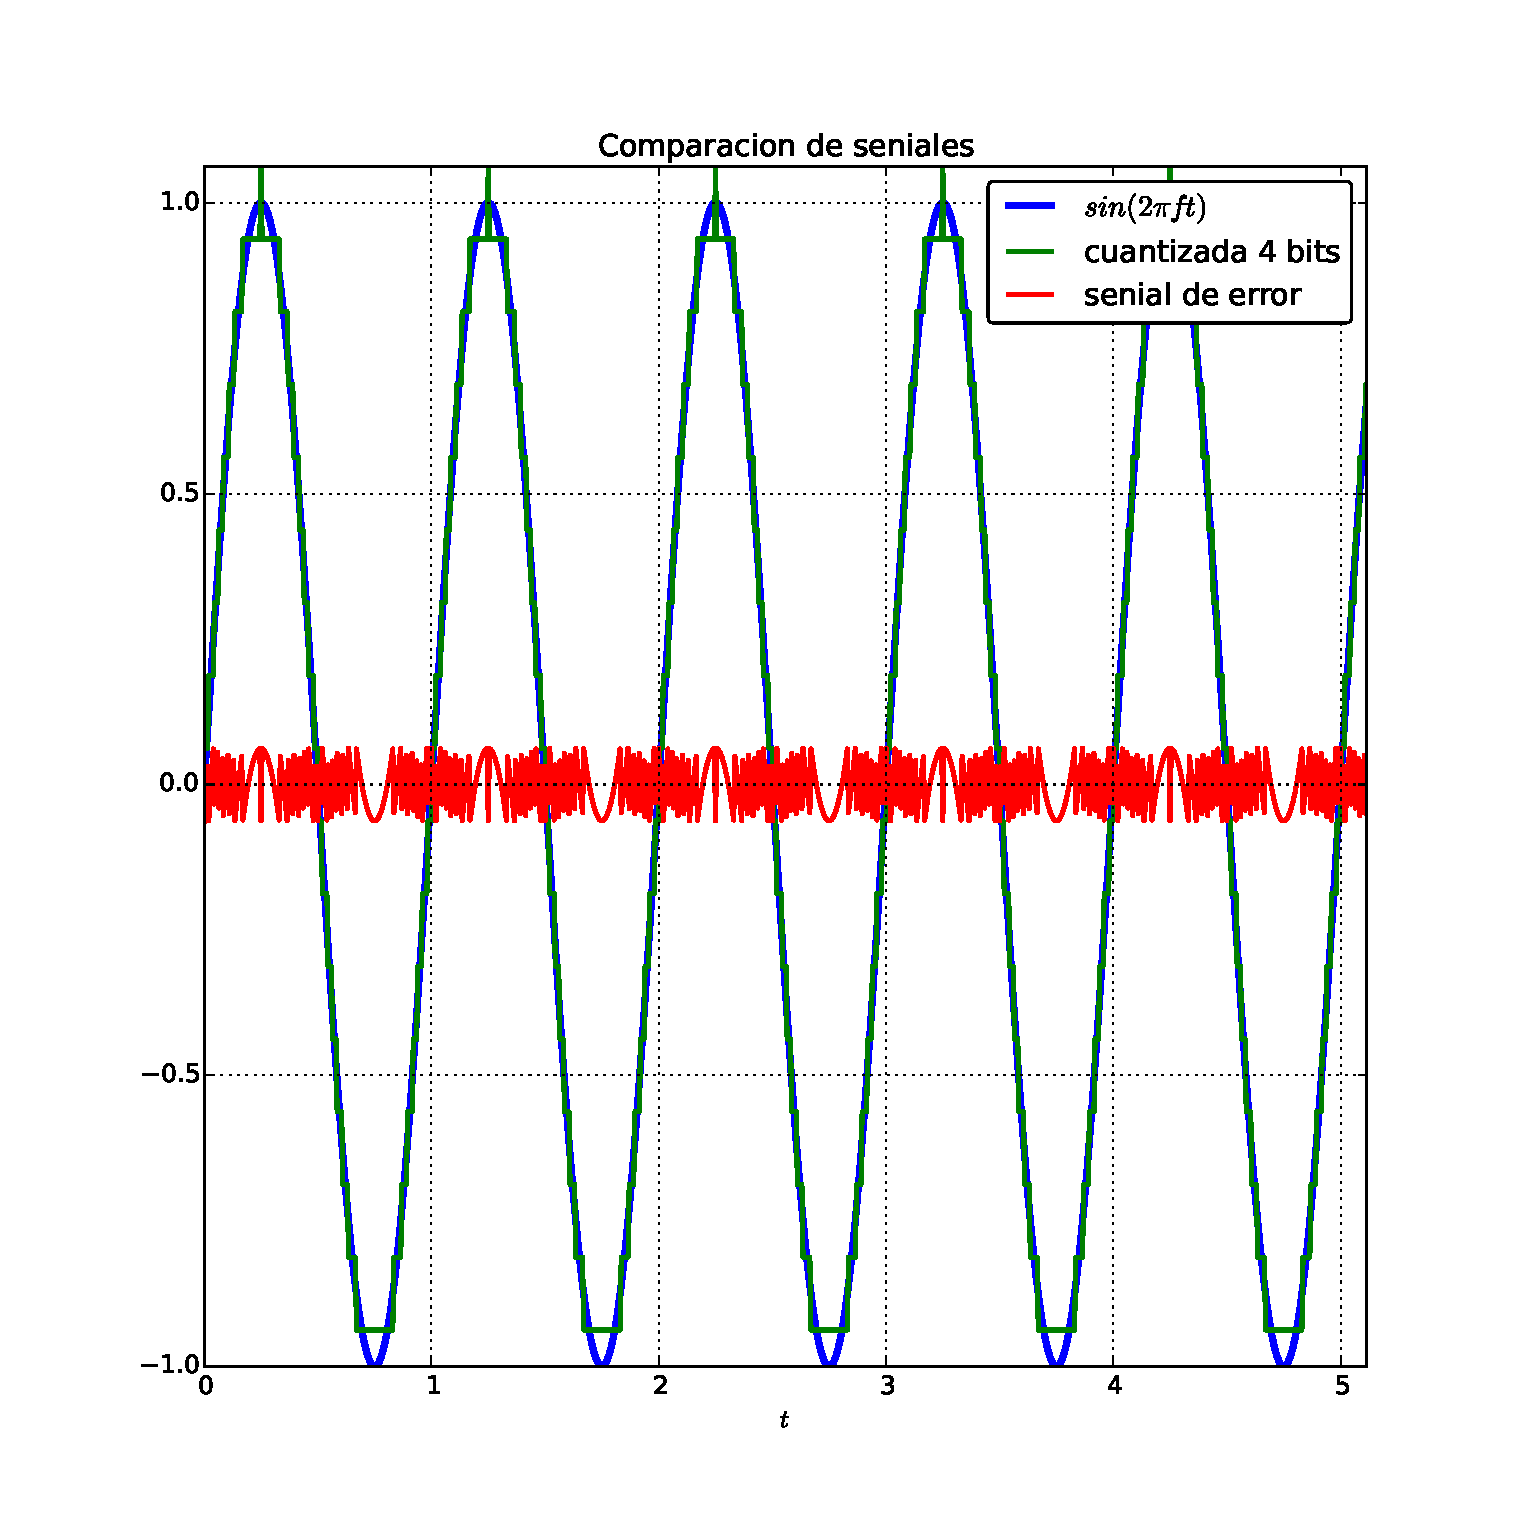
\includegraphics[width=0.48\textwidth]{./Images/seniales_4_bits.eps}
   \caption{Cuantización 4 bits}\label{fig:q:4}     
\end{figure}


\begin{figure}[H]
   \centering
   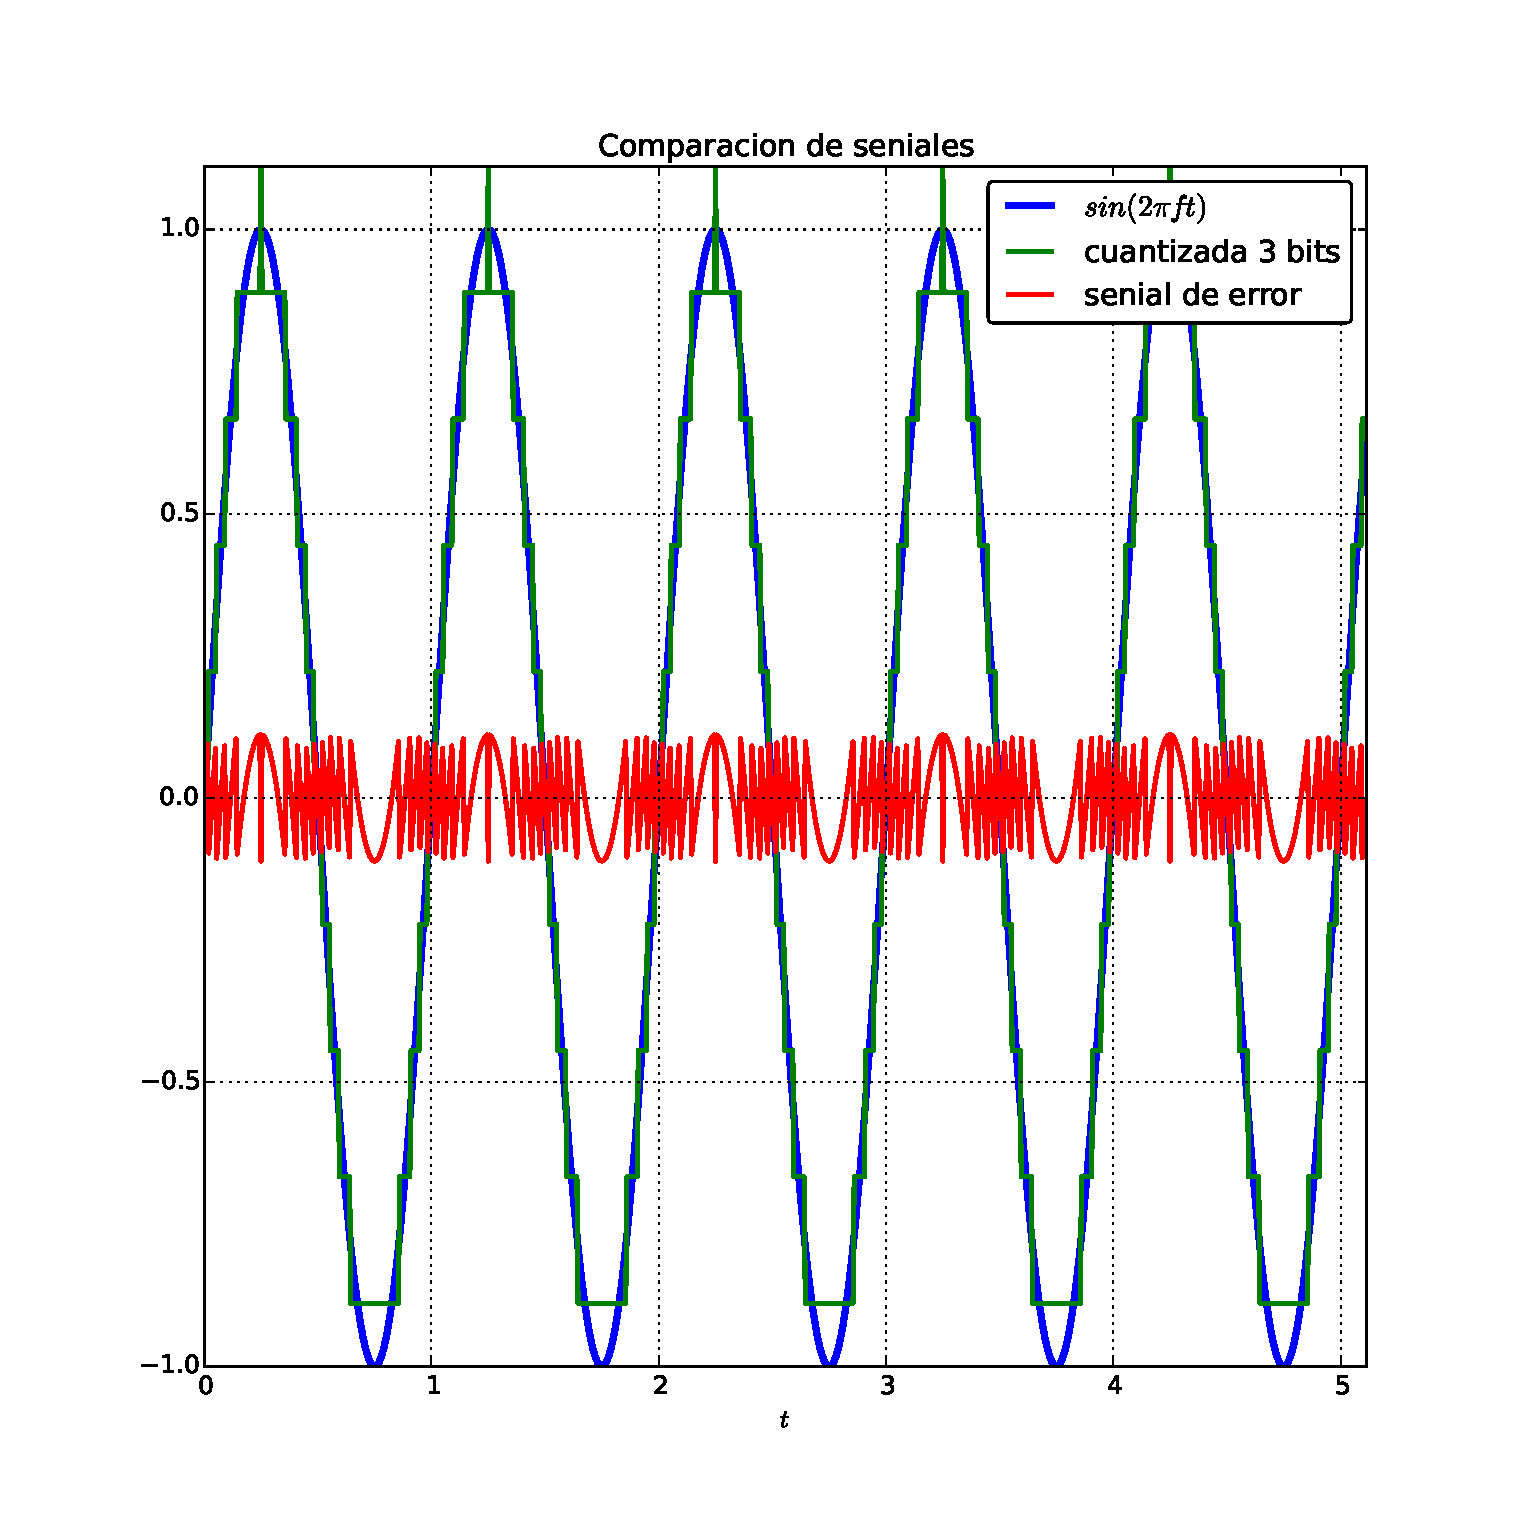
\includegraphics[width=0.48\textwidth]{./Images/seniales_3_bits.eps}
   \caption{Cuantización 3 bits}\label{fig:q:3}     
\end{figure}


\begin{figure}[H]
   \centering
   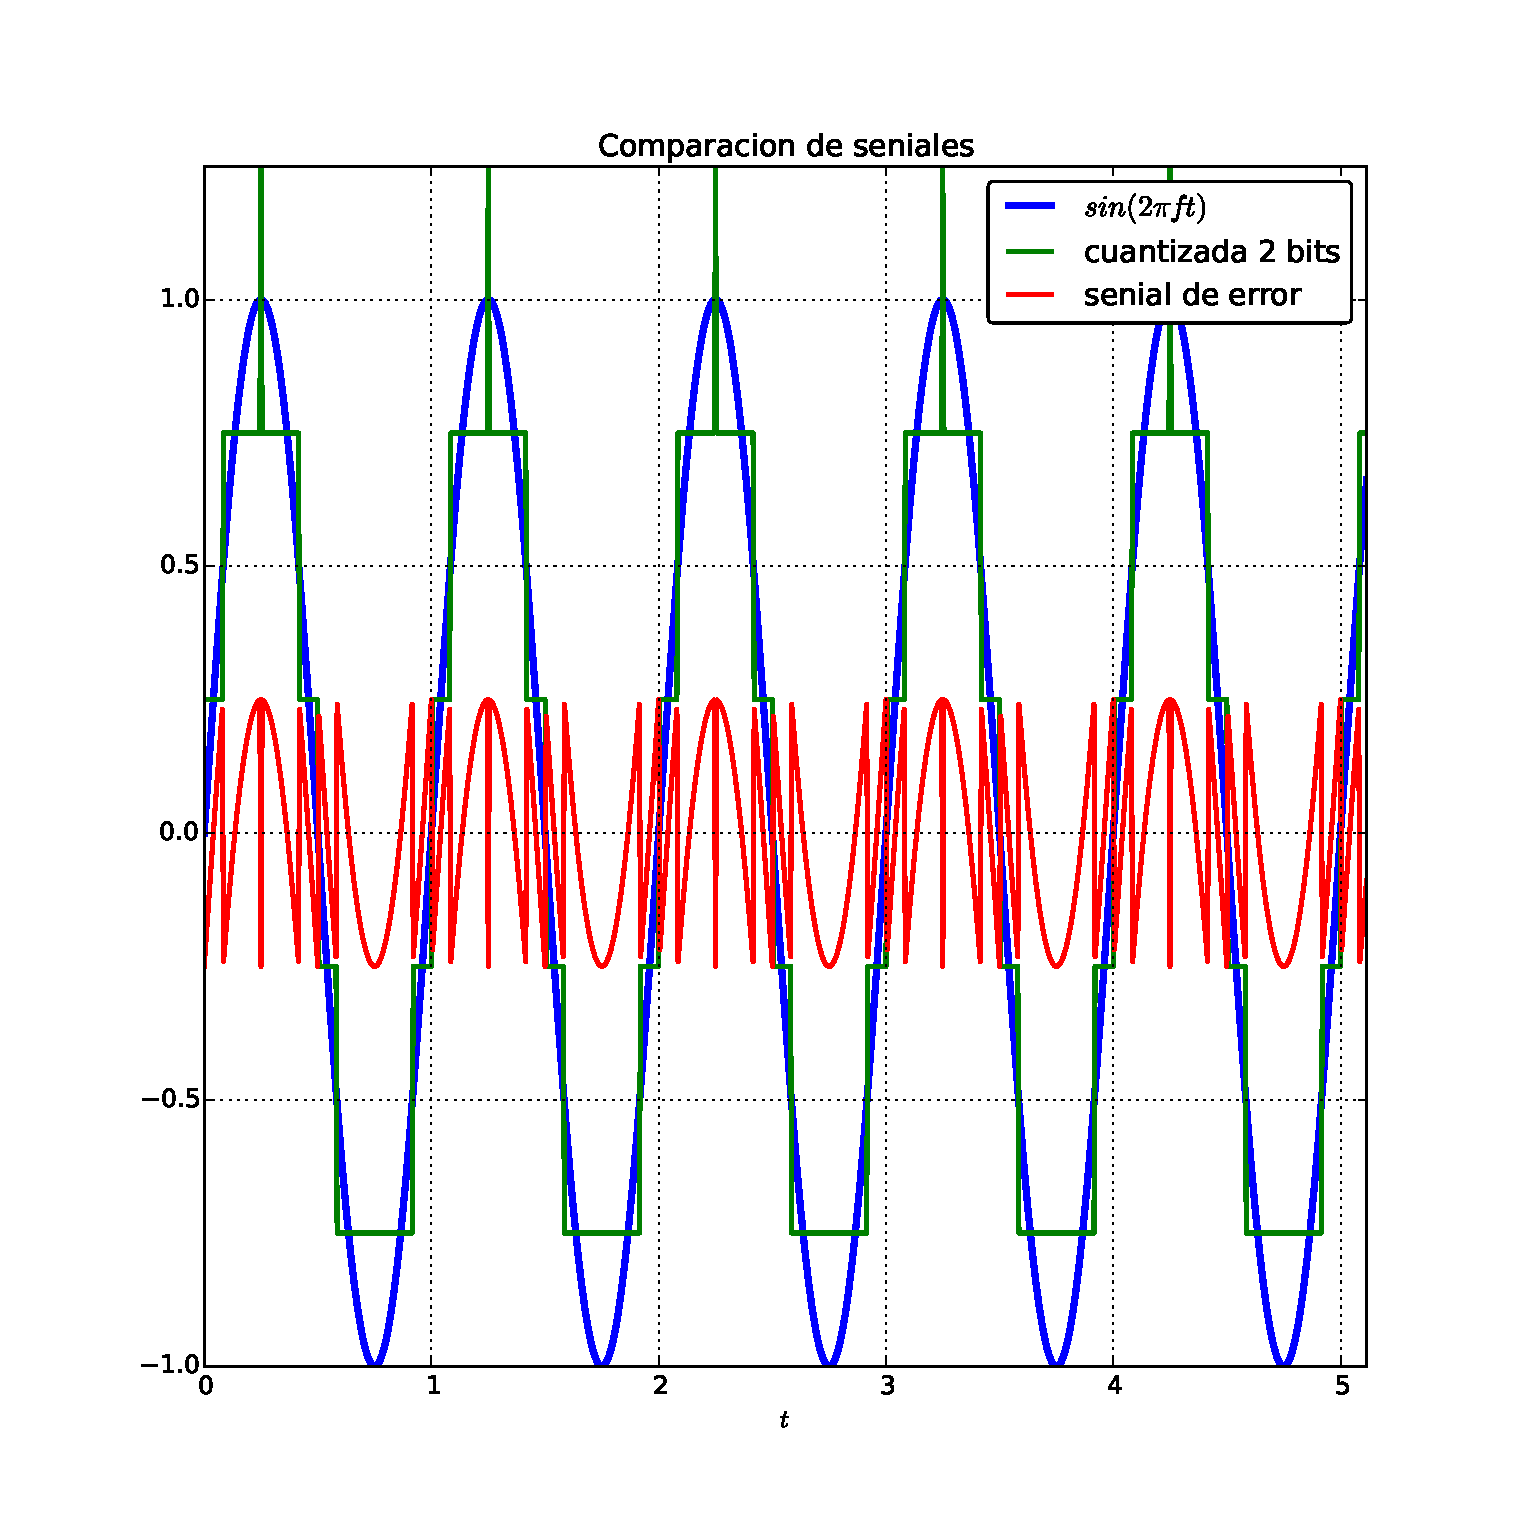
\includegraphics[width=0.48\textwidth]{./Images/seniales_2_bits.eps}
   \caption{Cuantización 2 bits}\label{fig:q:2}     
\end{figure}

Como se puede apreciar la señal de error $e(t)=x-x_{q_{i}}$ tiene amplitud más grande
al cuantizar a la señal original con menos niveles.

\section{Problema 5}
Se propone ahora simular los efectos de la cuantización uniforme sobre una señal
de voz (tomada de algún archivo de audio de pocos segundos de duración muestreada
con n bits de manera que su calidad sea media).
A partir de una señal de voz original se pide cuantizar la señal con menos bits que la
original

\begin{itemize}
    \item a- Medir la SNR para cada uno de los casos anteriores y reproducir la señal cuantizada en la tarjeta de audio. Comentar los resultados.
\end{itemize}

\subsection{resolución}
Nuevamente se realizó un script(\verb|problema5.jl|) que realiza la lectura-escritura de los archivos \verb|wav|
y además comparamos gráficamente todas las seniales. A continuación las salidas del mencionado script.


\begin{figure}[H]
   \centering
   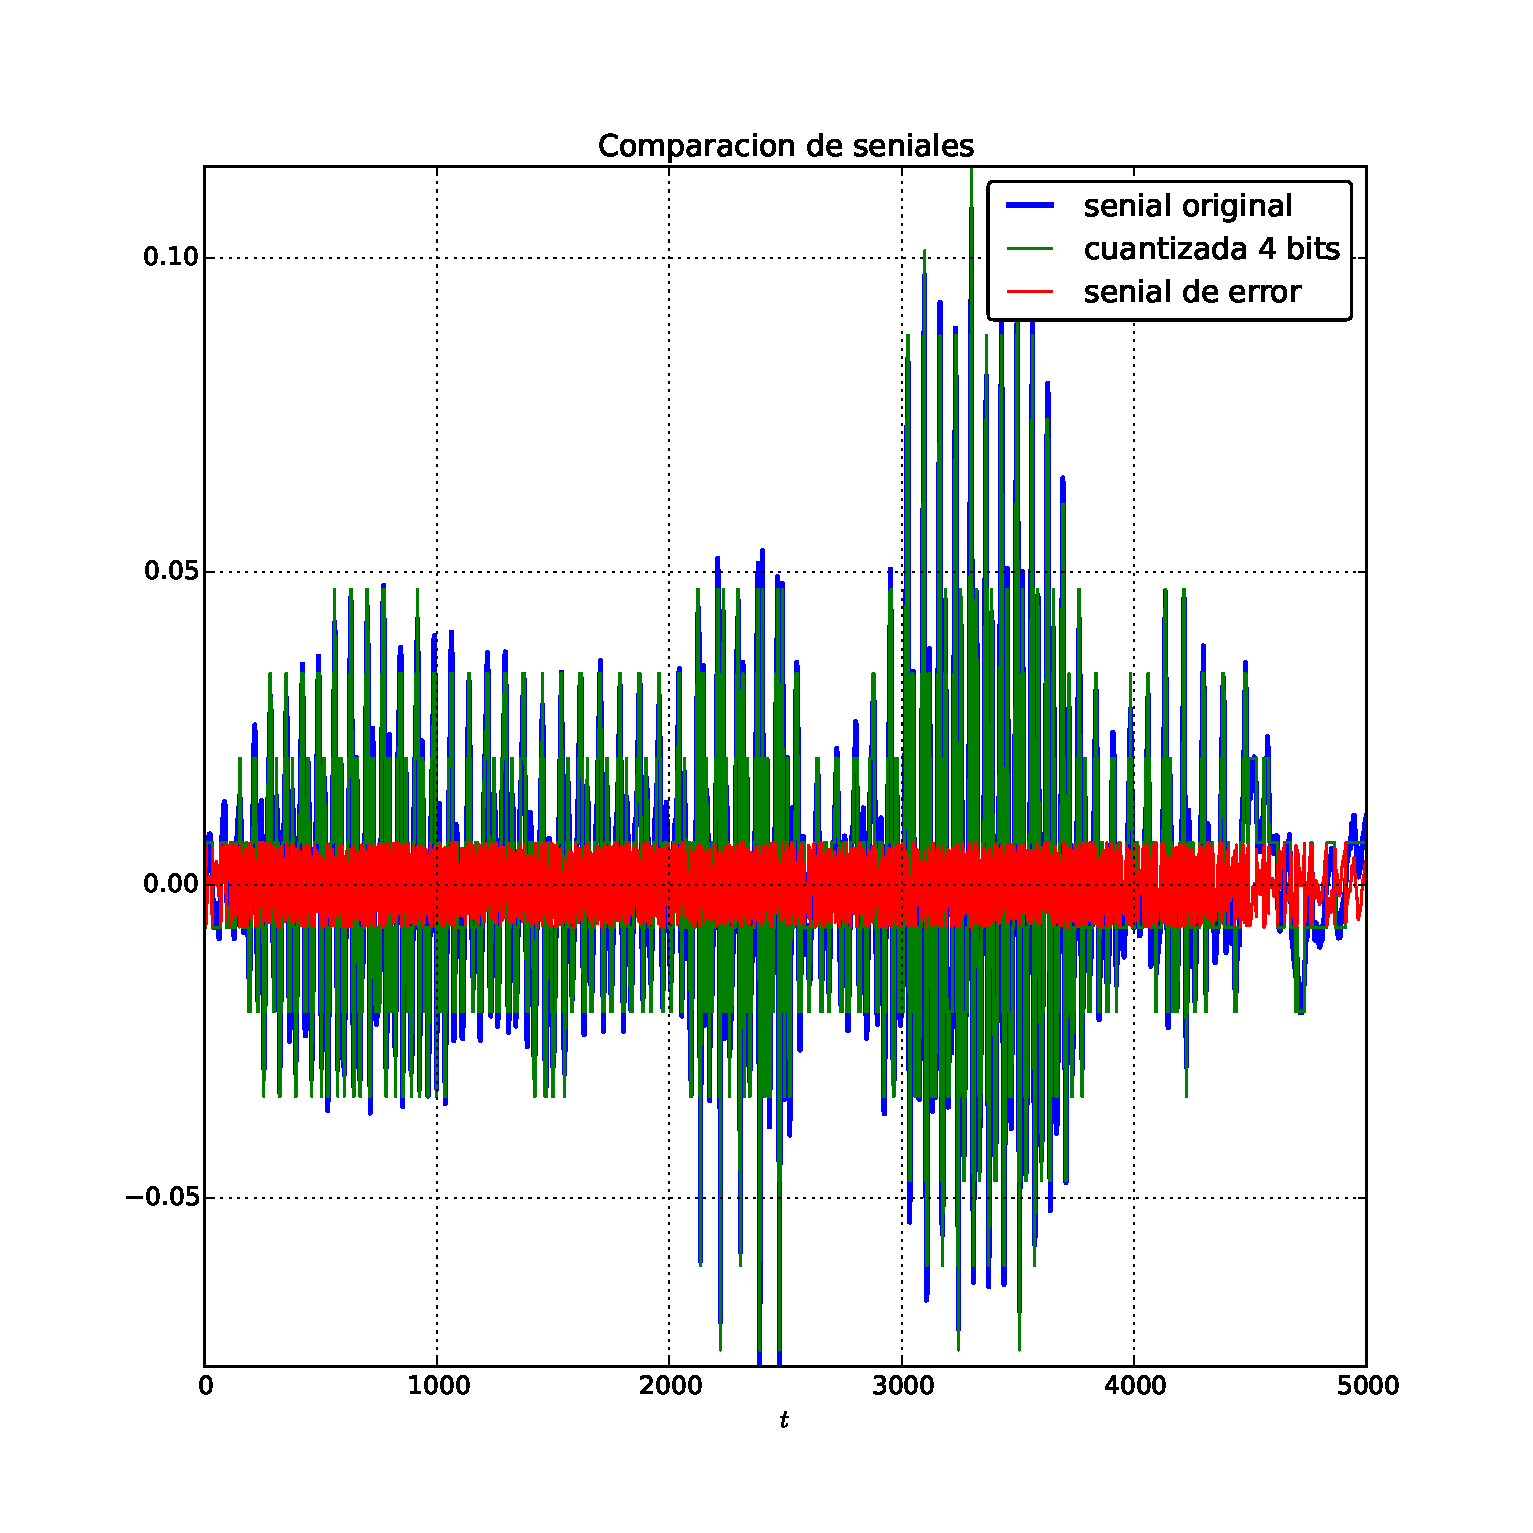
\includegraphics[width=0.48\textwidth]{./Images/senialesv_voz_4_bits.eps}
   \caption{Cuantización 4 bits}\label{fig:qv:4}     
\end{figure}


\begin{figure}[H]
   \centering
   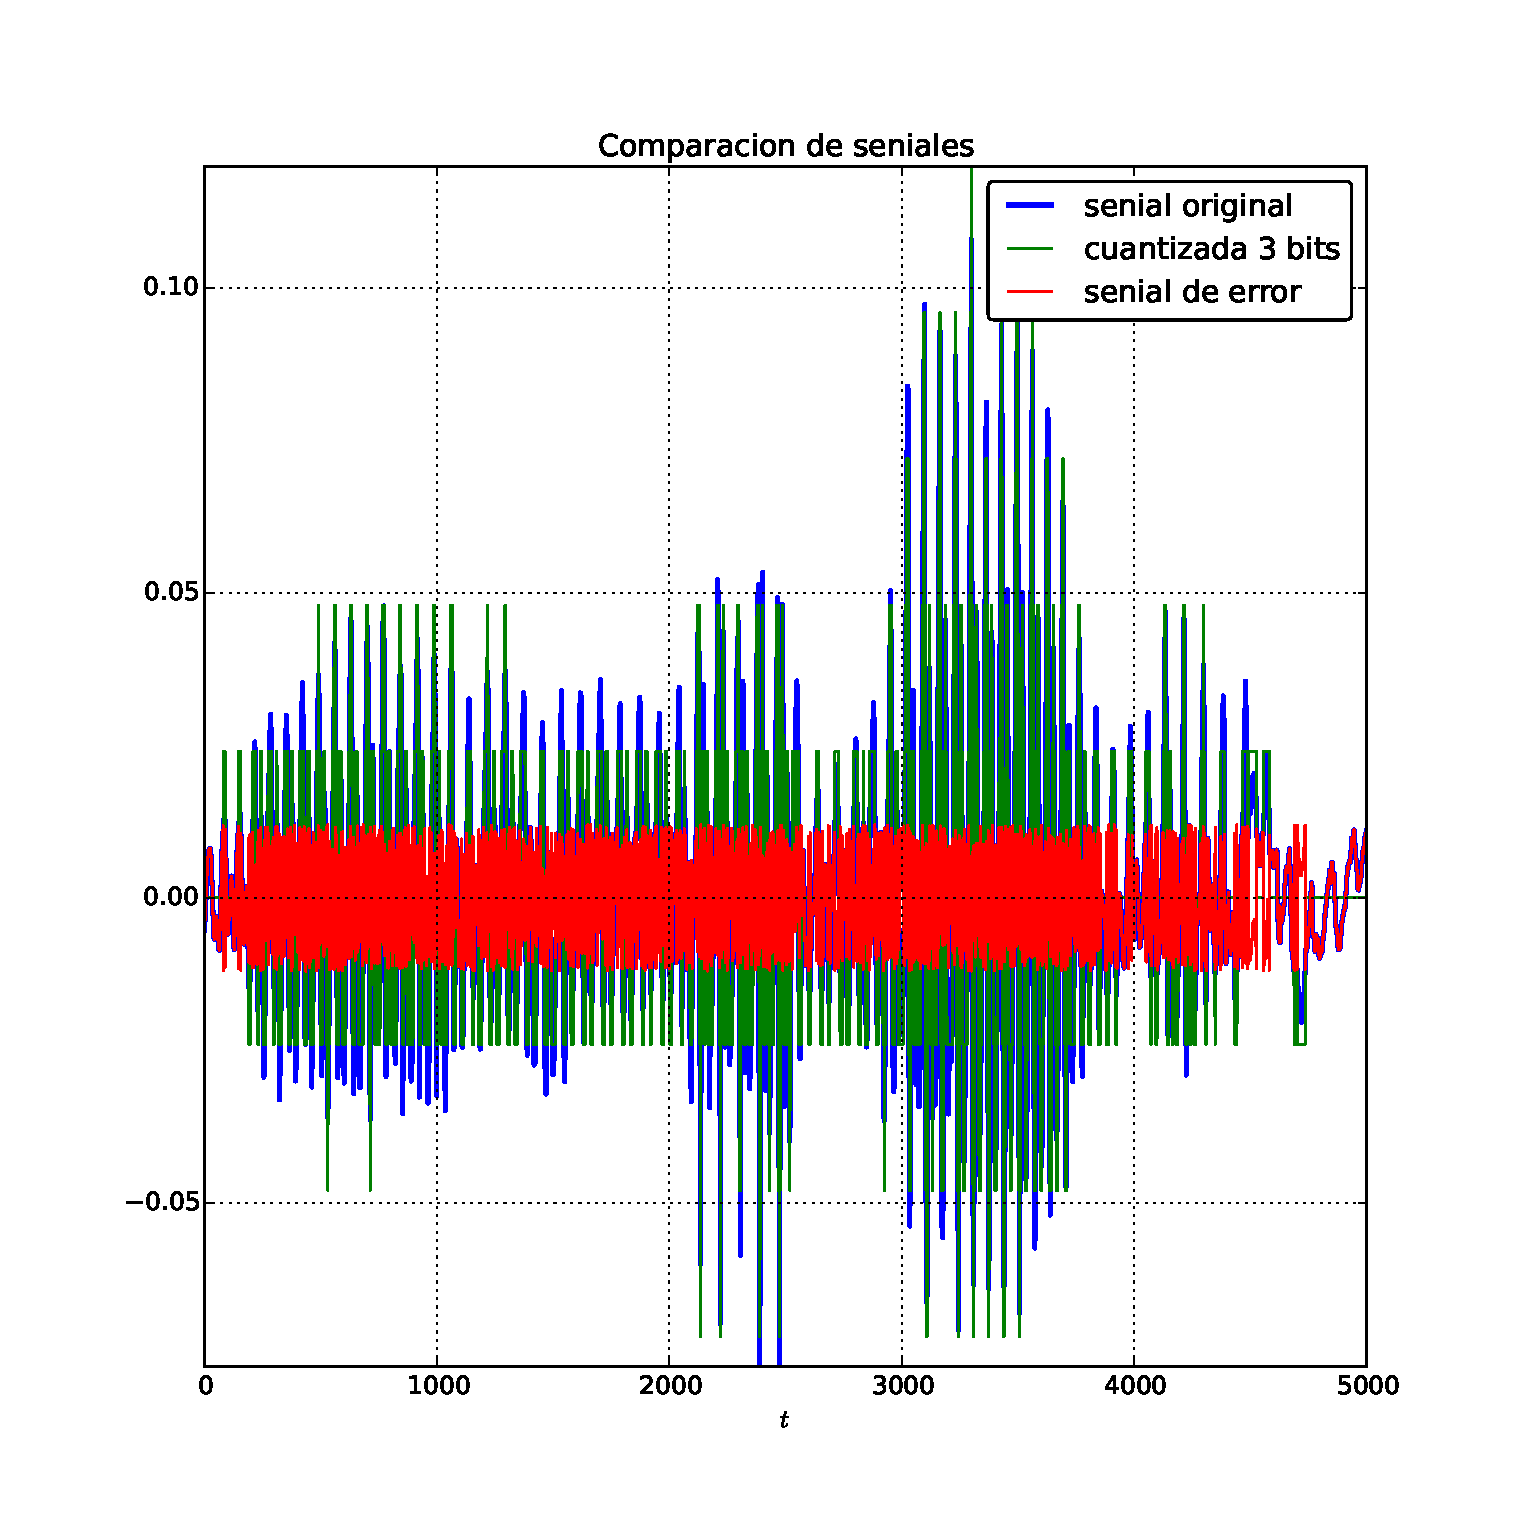
\includegraphics[width=0.48\textwidth]{./Images/senialesv_voz_3_bits.eps}
   \caption{Cuantización 3 bits}\label{fig:qv:3}     
\end{figure}


\begin{figure}[H]
   \centering
   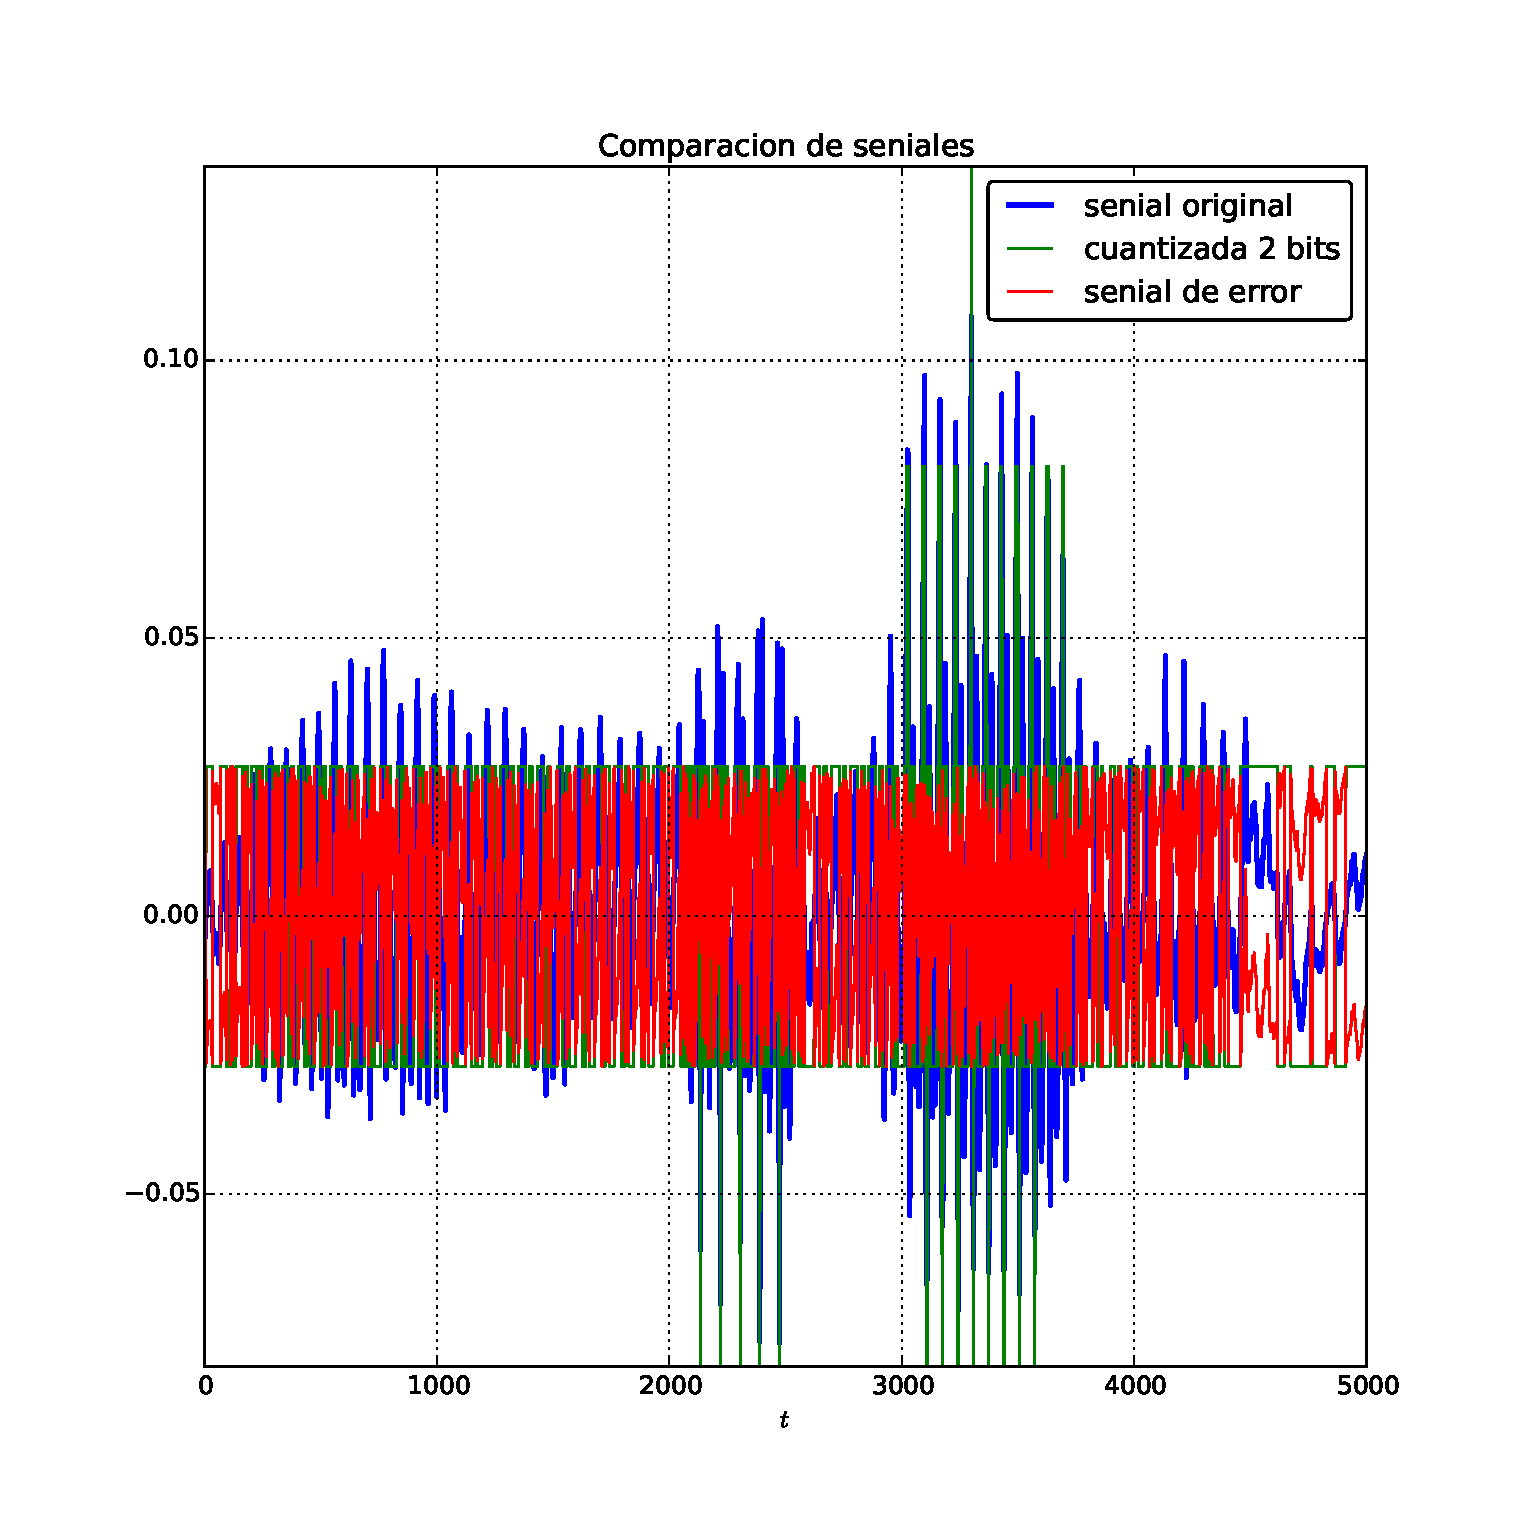
\includegraphics[width=0.48\textwidth]{./Images/senialesv_voz_2_bits.eps}
   \caption{Cuantización 2 bits}\label{fig:qv:2}     
\end{figure}
La relación senial-ruido para una senial cuantizada uniformemente se puede expresar:
\begin{equation}
\Bigg( \frac{S}{N} \Bigg)_{q} = \frac{L^{2}q^{2}/4}{q^{2}/12} = 3L^{2}
\end{equation}
Donde $L$ son los números de niveles de cuantización.

Por ello para 2 bits de resolución tenemos(en $[Db]$):

\verb|julia> 10*log10(12*1^2/2/(2/4)^2)|\\
\verb|13.80211241711606|\\
para 3 bits\\
\verb|julia>10*log10(12*1^2/2/(2/8)^2)|\\
\verb|19.822712330395685|\\
para 4 bits\\
\verb|julia>10*log10(12*1^2/2/(2/16)^2)|\\
\verb|25.84331224367531|\\

A la salida del script obtemos:
\begin{verbatim}
julia> include("problema5.jl")
WARNING: replacing module Teleco2
La relación senial-ruido para 2 bits es: 4.7383394267141[Db]
La relación senial-ruido para 3 bits es: 9.682605271481124[Db]
La relación senial-ruido para 4 bits es: 20.744776704544634[Db]
\end{verbatim}

Como sabemos las seniales de voz estadisticamente tienen amplitudes bajas, osea que
los niveles altos de voz son pocos probables, de alli que para esta senial de 
voz obtenemos resultados distintos de los teoricos que modelan a la probabilidad 
de $p(q)=1/q$ además si tomamos como indicador de como se
degrada la senial de acuerdo a la varianza del error producido por el redondeo, vimos que
la varianza $\sigma^{2}=\frac{q^{2}}{12}$ se corresponde con la potencia media de ruido 
a la cuantización. Por ello como podemos ver en la cuantización uniforme el ruido se mantiene constante
ya que $q$ es constante, pero como los niveles de amplitud no entonces la relación senial-ruido varía. 

\section{Problema 6}
Modificando el diagrama utilizado en la simulación de la cuantización uniforme para
señales de voz para implementar el cuantizador ley-$\mu$.
\begin{itemize}
\item a- Medir la SNR para cada uno de los casos (cuantización de 4, 3 y 2 bits) y
reproducir la señal cuantizada en la tarjeta de audio.
\item b- Modificar el esquema y adicionar dos “SCOPE”, uno antes de comprimir la
señal con un filtro con ley-$\mu$ y otro posterior al filtro con ley-$\mu$.
Sacar conclusiones en base a lo visualizado.
\item c- Comparar con los resultados del cuantizador uniforme y sacar
conclusiones.
\item d- Graficar la Densidad Espectral de la Señal (Utilizando Matlab) y Sacar
Conclusiones:
\begin{itemize}
\item A la entrada del Sistema.
\item A la salida del filtro ley-$\mu$.
\item A la salida del Sistema.
\end{itemize}
\end{itemize}
\subsection{resolución}

Nuevamente se realizó un script(\verb|problema6.jl|) que realiza la lectura-escritura de los archivos \verb|wav|
y además comparamos gráficamente todas las seniales. A continuación las salidas del mencionado script.

\begin{verbatim}
julia> include("problema6.jl")
La relación senial-ruido para 2 bits es: 4.994832156111841 [Db]
La relación senial-ruido para 3 bits es: 9.01438241013517 [Db]
La relación senial-ruido para 4 bits es: 26.059268713048507 [Db]
\end{verbatim}

\begin{figure}[H] 
\centering
   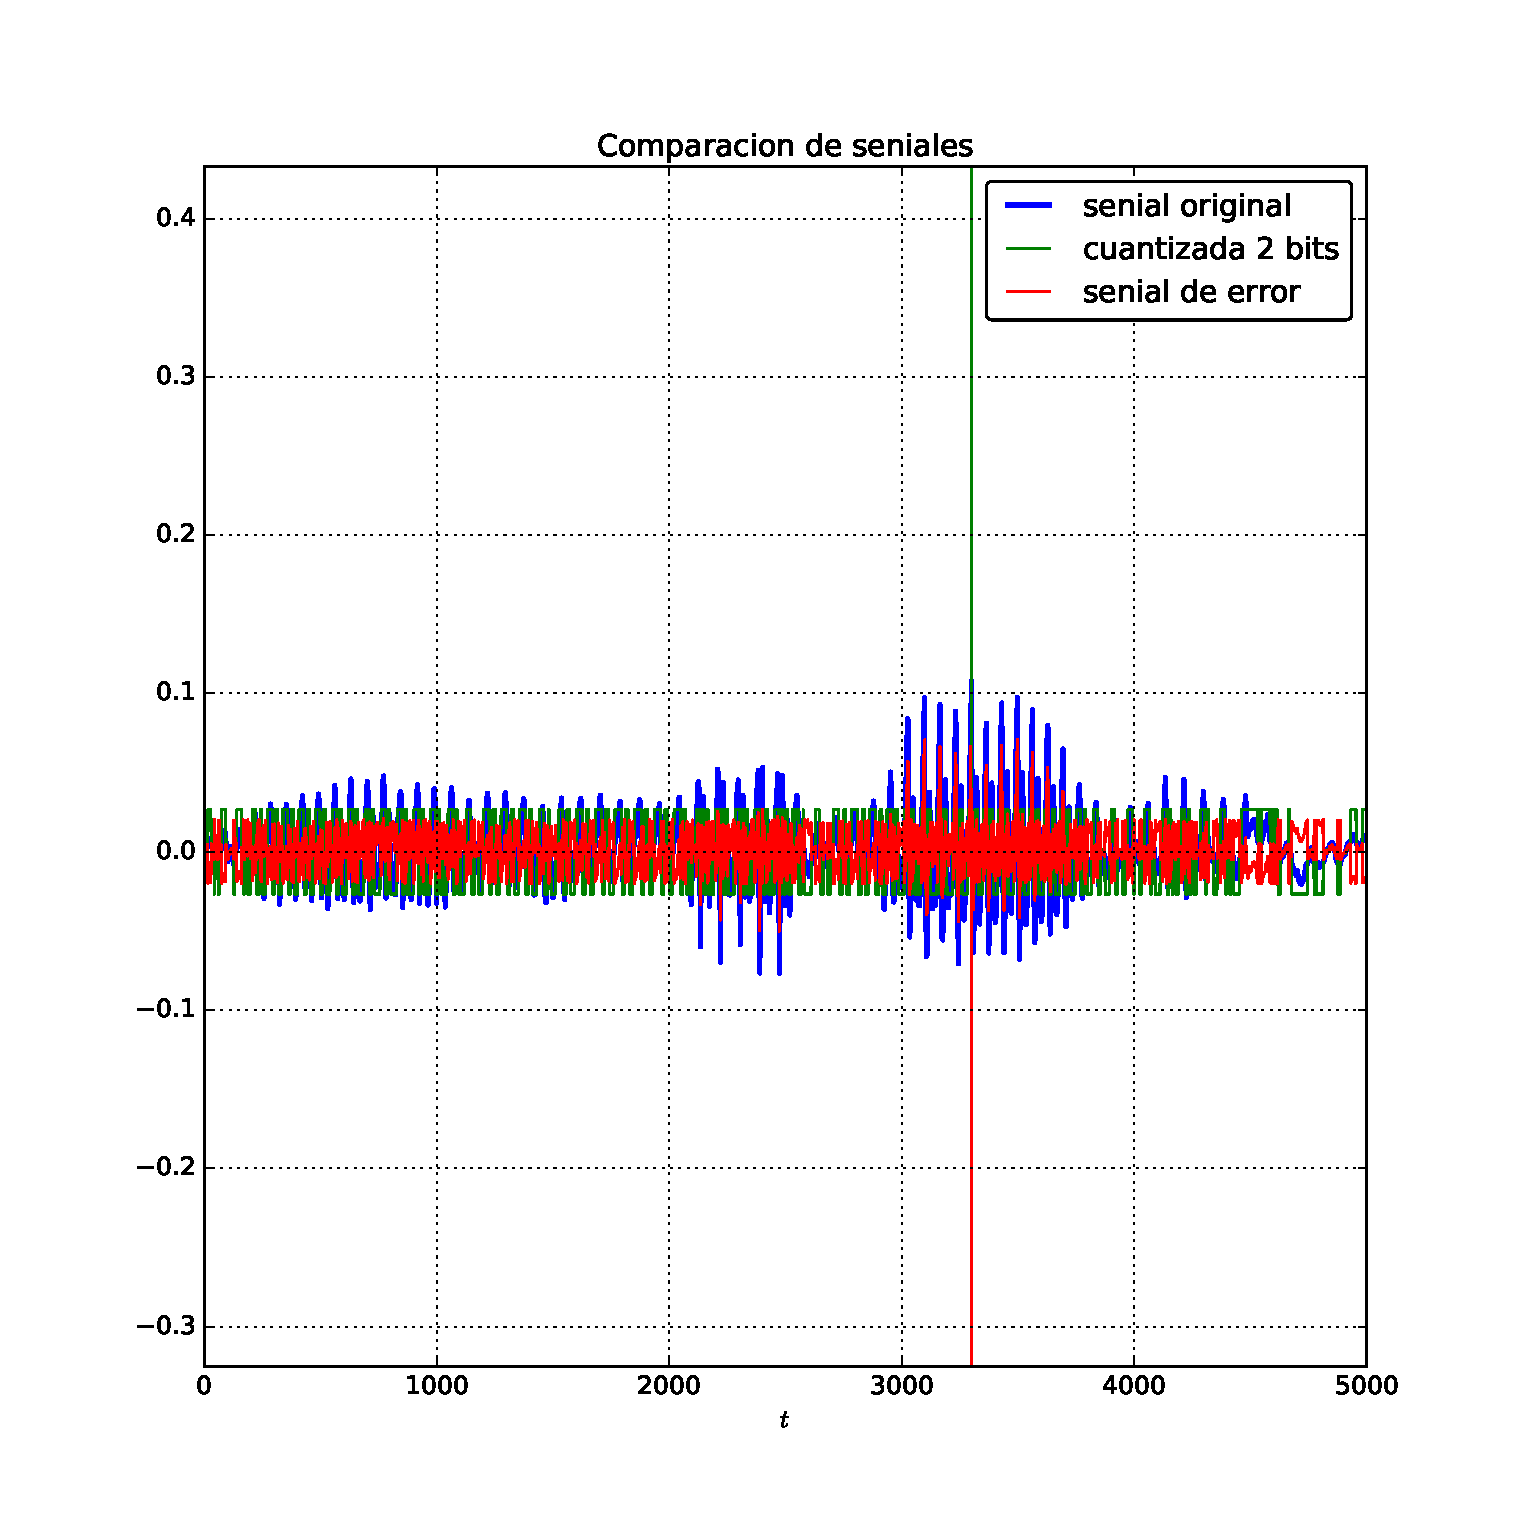
\includegraphics[width=0.48\textwidth]{./Images/senialesv_voz_2_bits_mu.eps}
   \caption{cuantización 2 bits con la ley-$\mu$}\label{fig:qv_mu:2}     
\end{figure}

\begin{figure}[H]
   \centering
   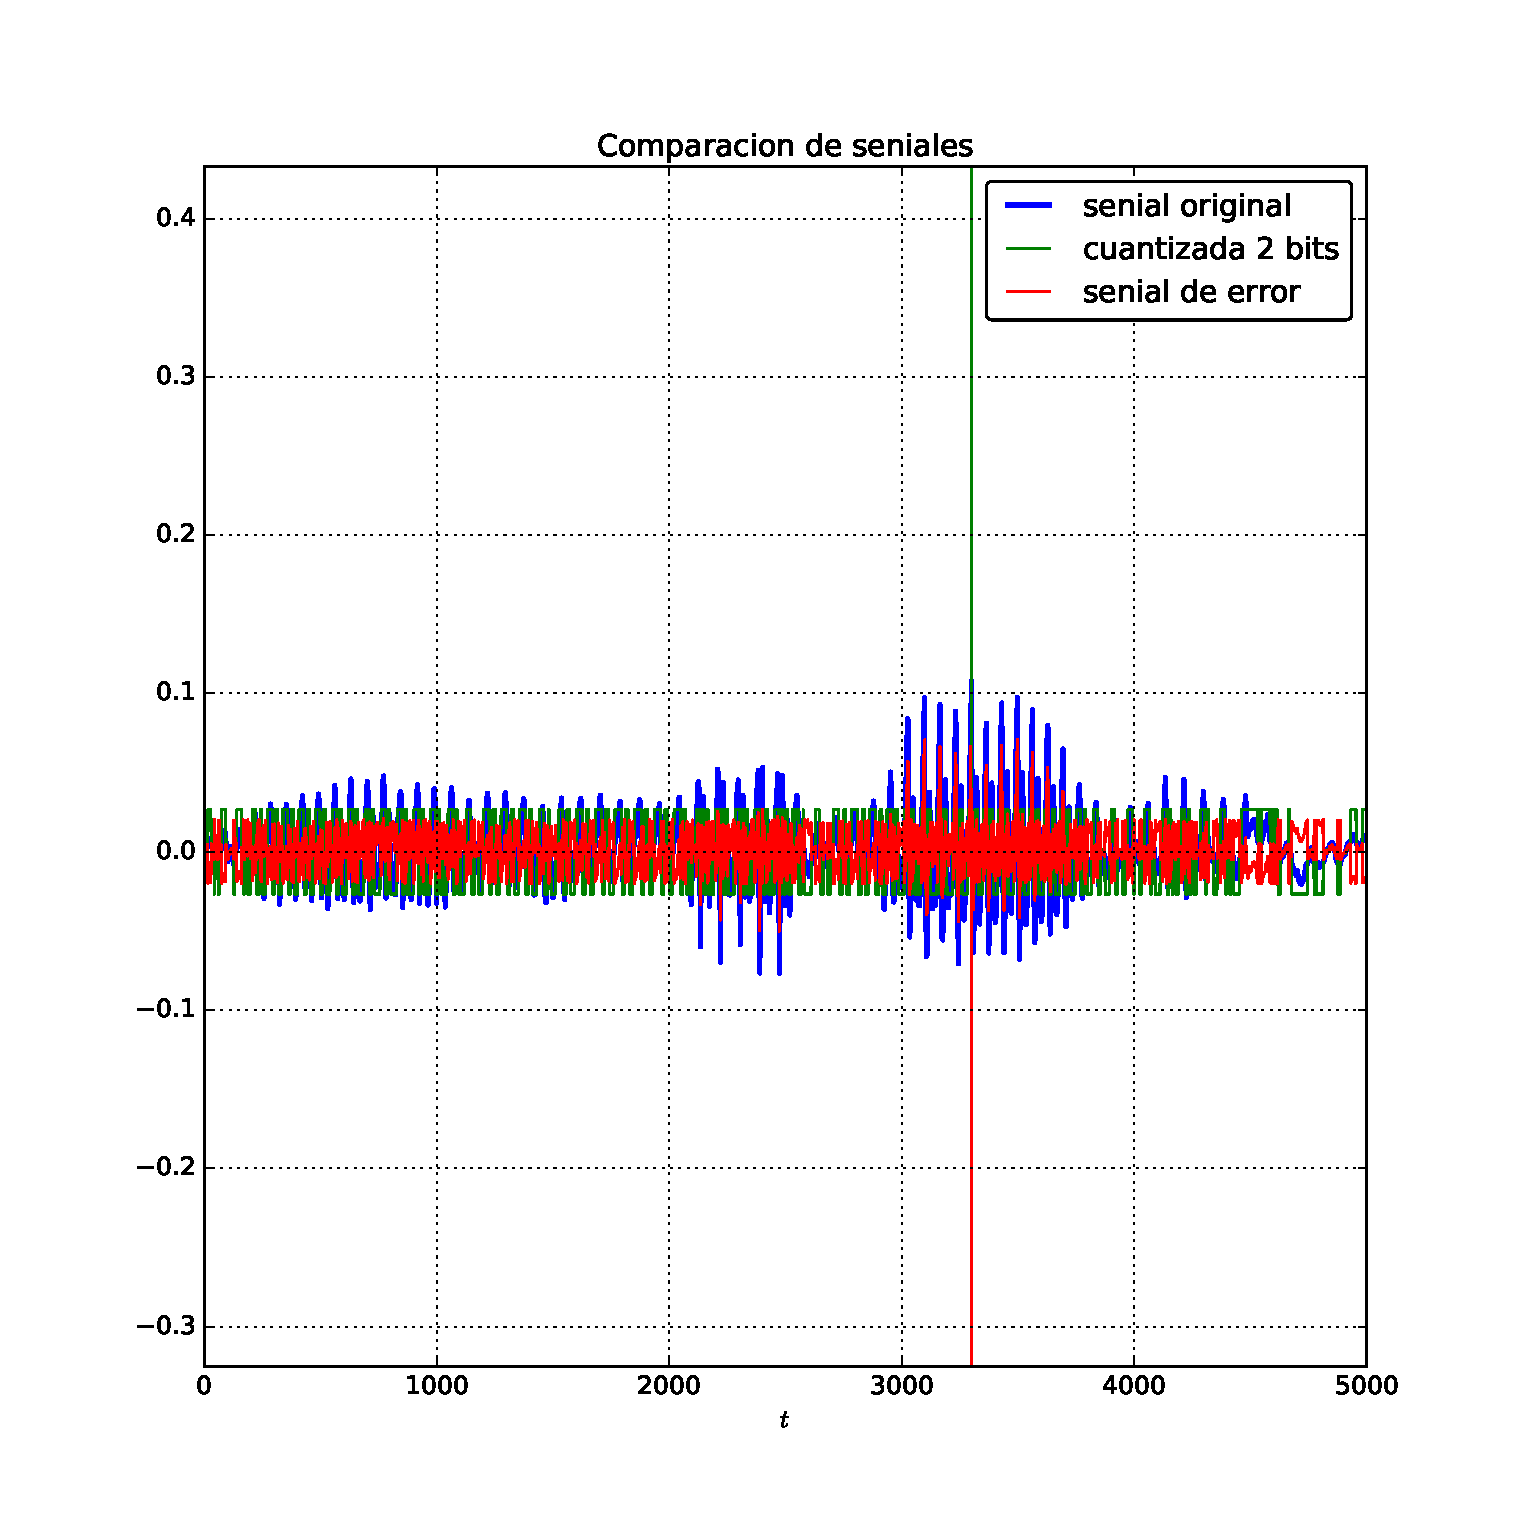
\includegraphics[width=0.48\textwidth]{./Images/senialesv_voz_2_bits_mu.eps}
   \caption{cuantización 3 bits con la ley-$\mu$}\label{fig:qv_mu:3}     
\end{figure}

\begin{figure}[H]
   \centering
   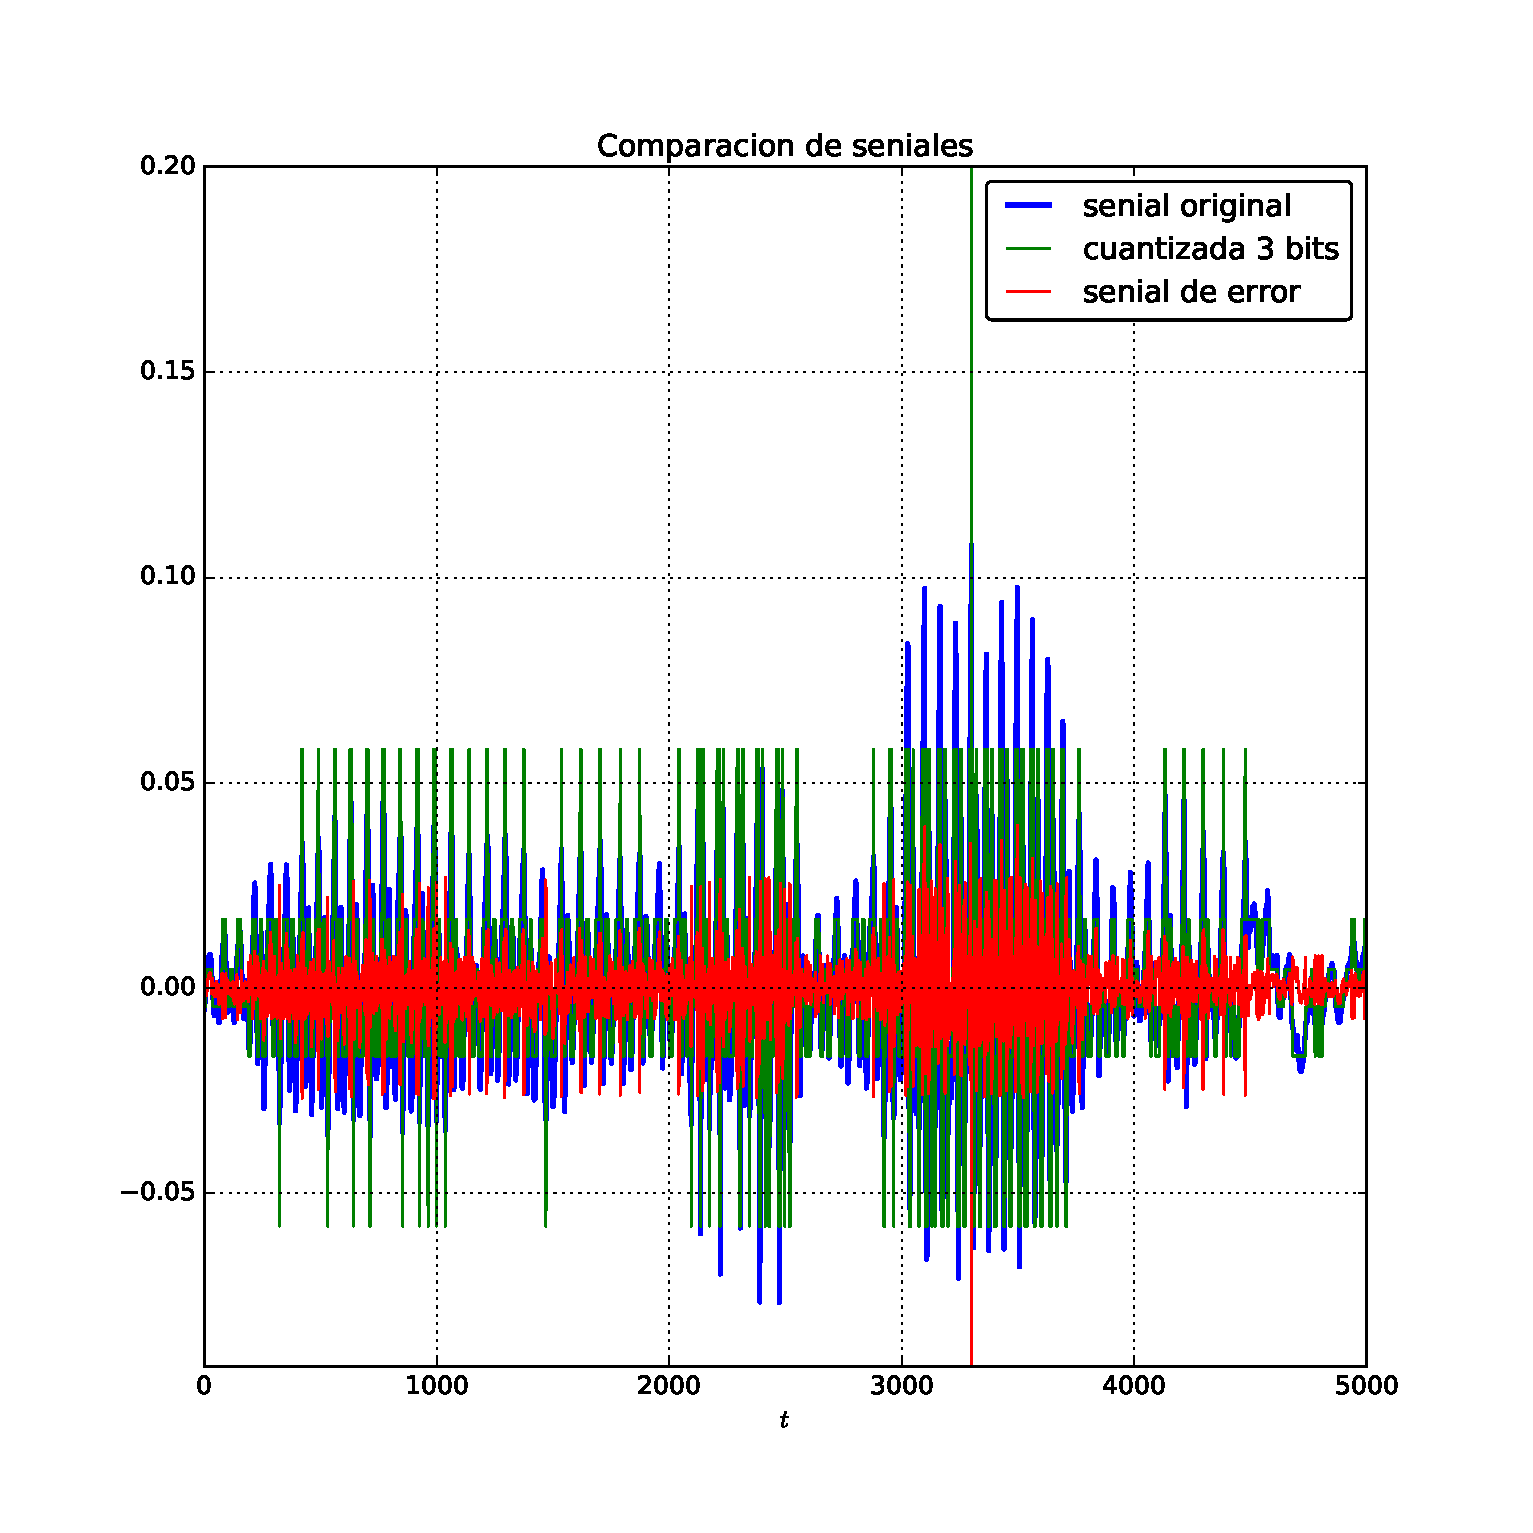
\includegraphics[width=0.48\textwidth]{./Images/senialesv_voz_3_bits_mu.eps}
   \caption{cuantización 4 bits con la ley-$\mu$}\label{fig:qv_mu:4}     
\end{figure}

\begin{figure}[H]
   \centering
   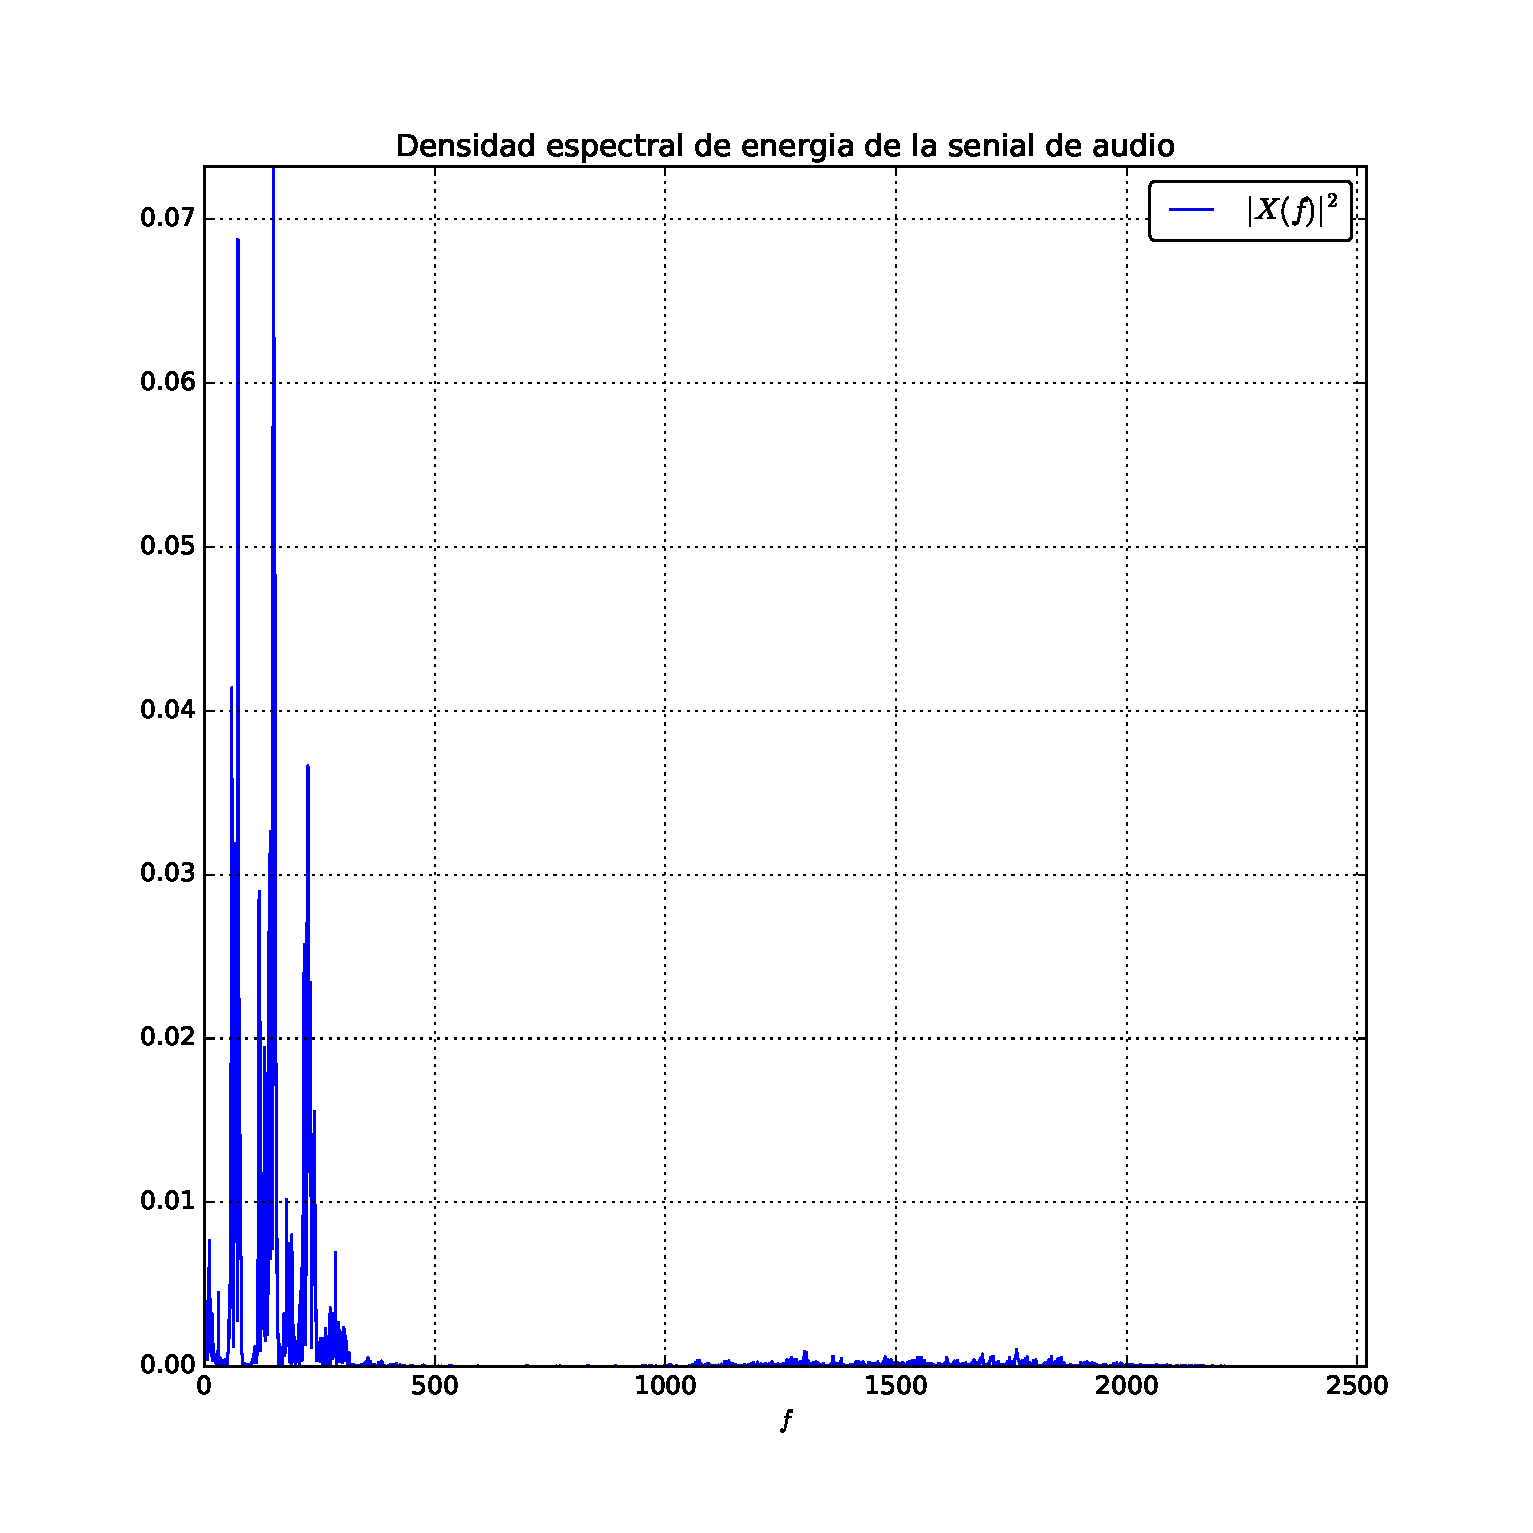
\includegraphics[width=0.48\textwidth]{./Images/densidad_espectral_x.eps}
   \caption{densidad espectral energia original}\label{fig:densidad}     
\end{figure}

\begin{figure}[H]
   \centering
   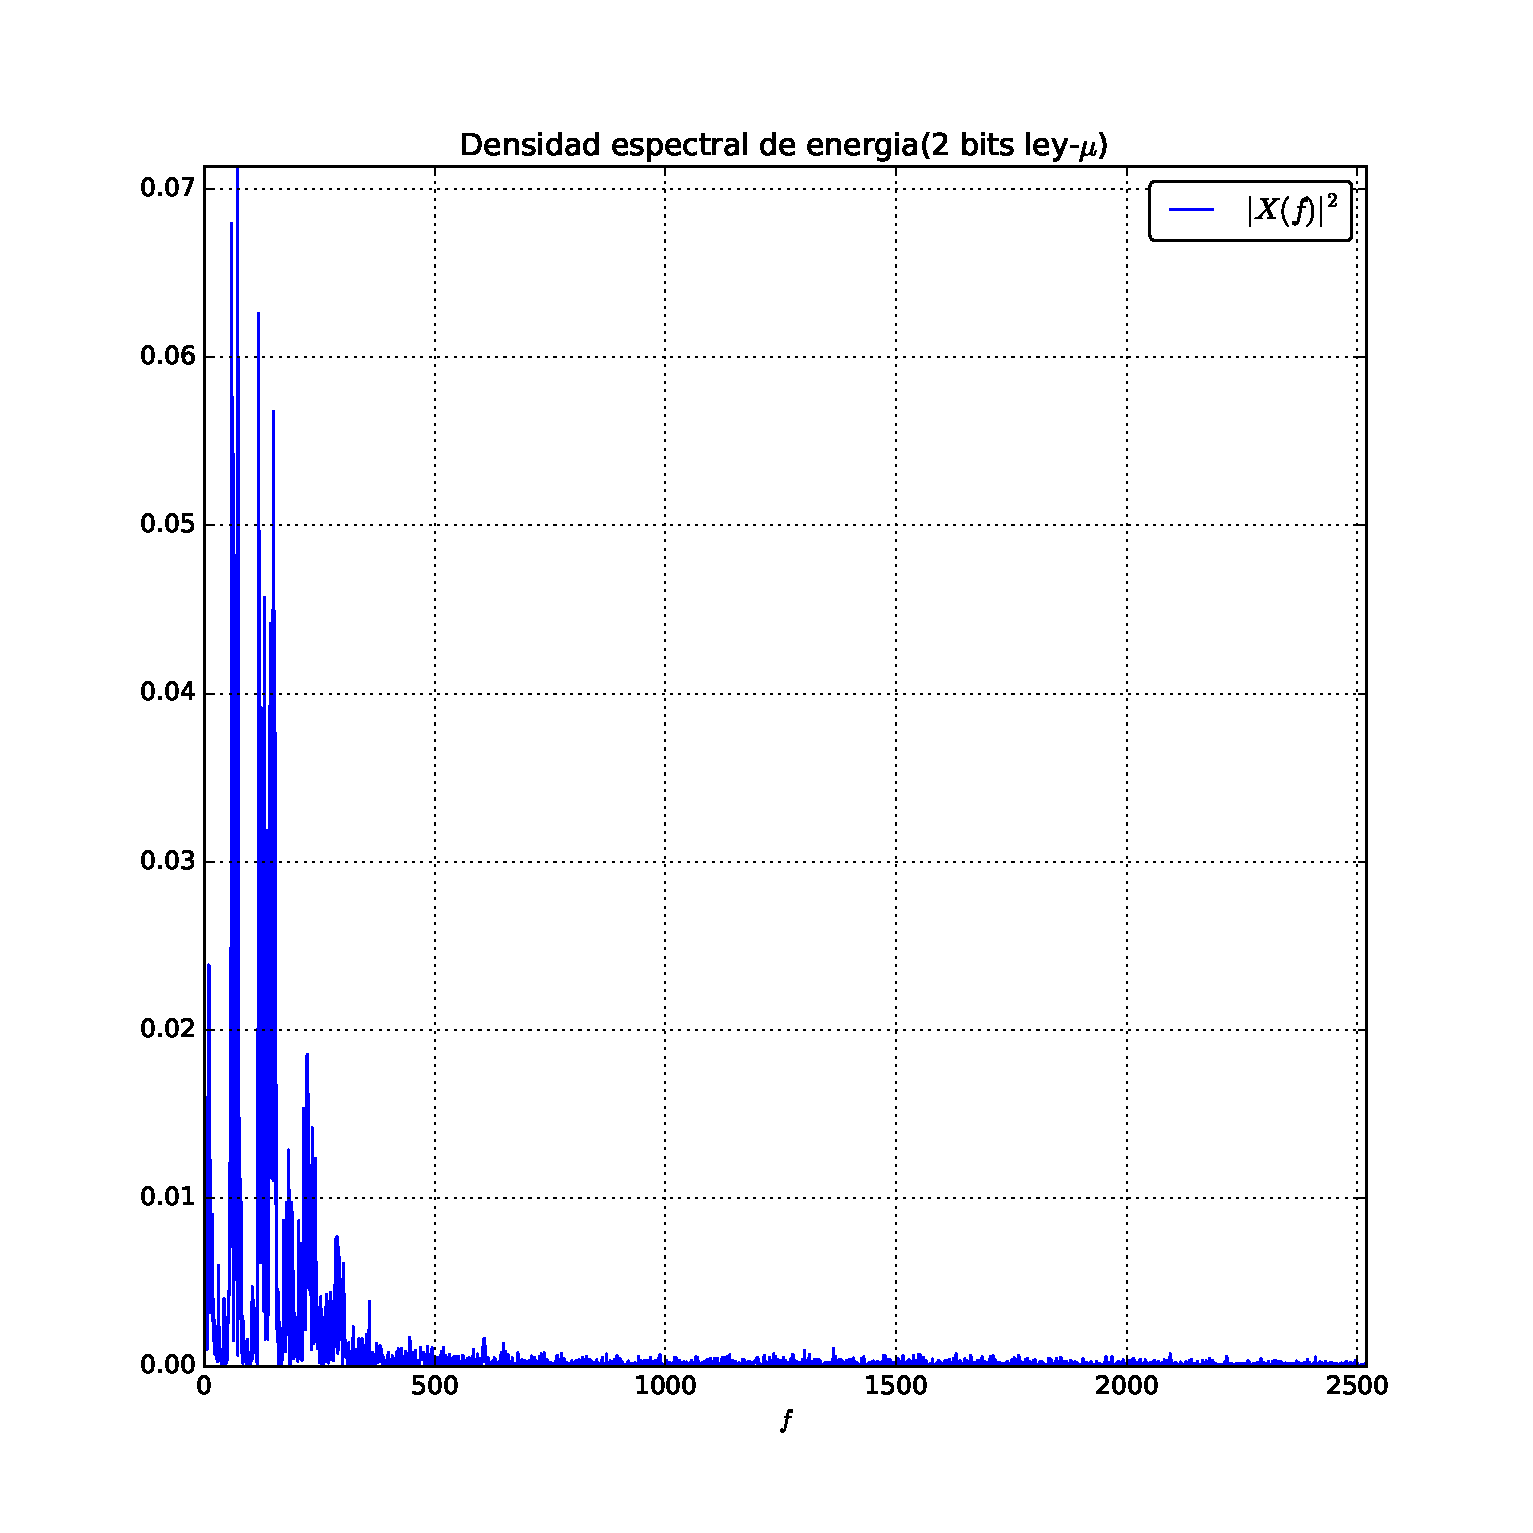
\includegraphics[width=0.48\textwidth]{./Images/densidad_espectral_x_2.eps}
   \caption{densidad espectral energia 2 bits}\label{fig:densidad_x_2}     
\end{figure}

\begin{figure}[H]
   \centering
   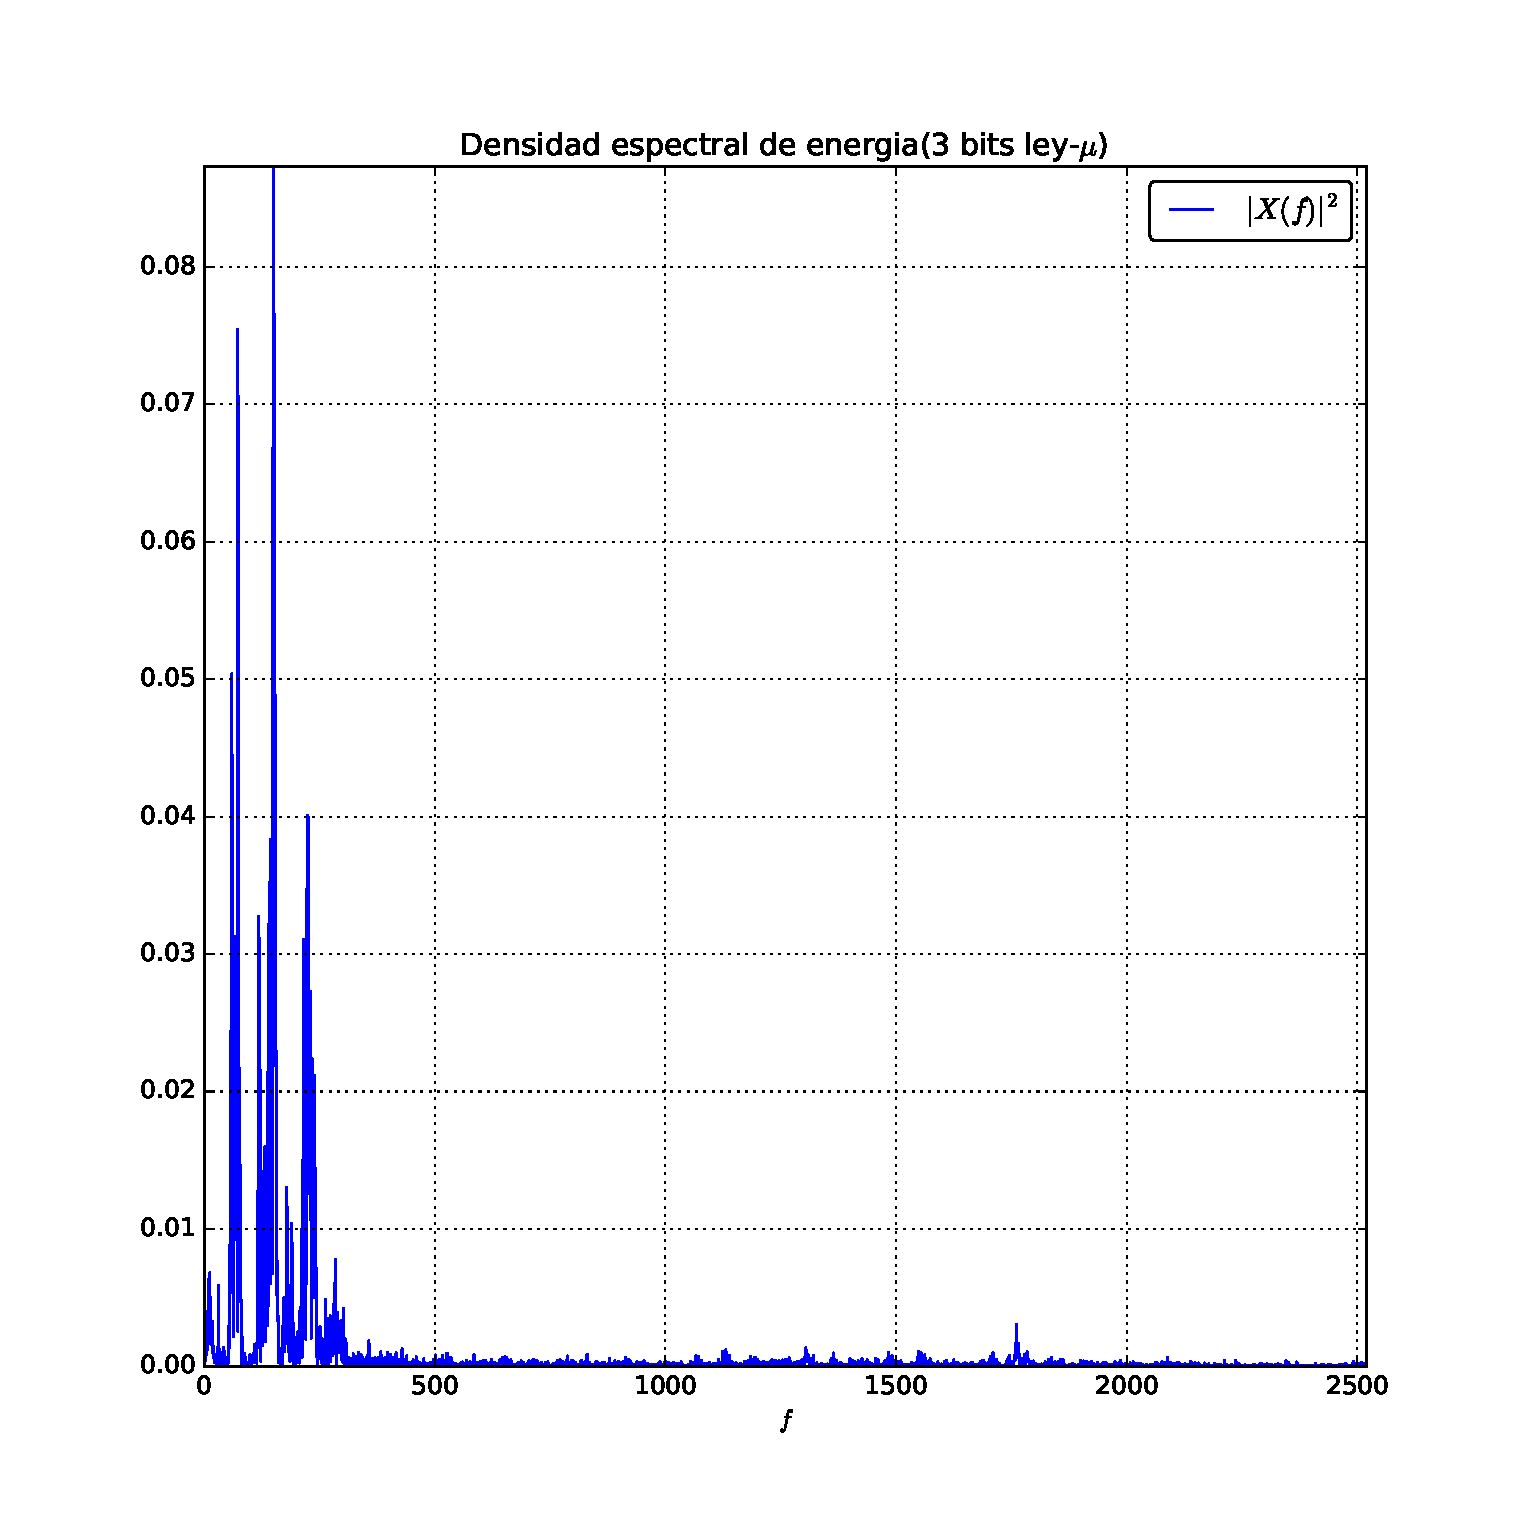
\includegraphics[width=0.48\textwidth]{./Images/densidad_espectral_x_3.eps}
   \caption{densidad espectral energia 3 bits}\label{fig:densidad_x_3}     
\end{figure}

\begin{figure}[H]
   \centering
   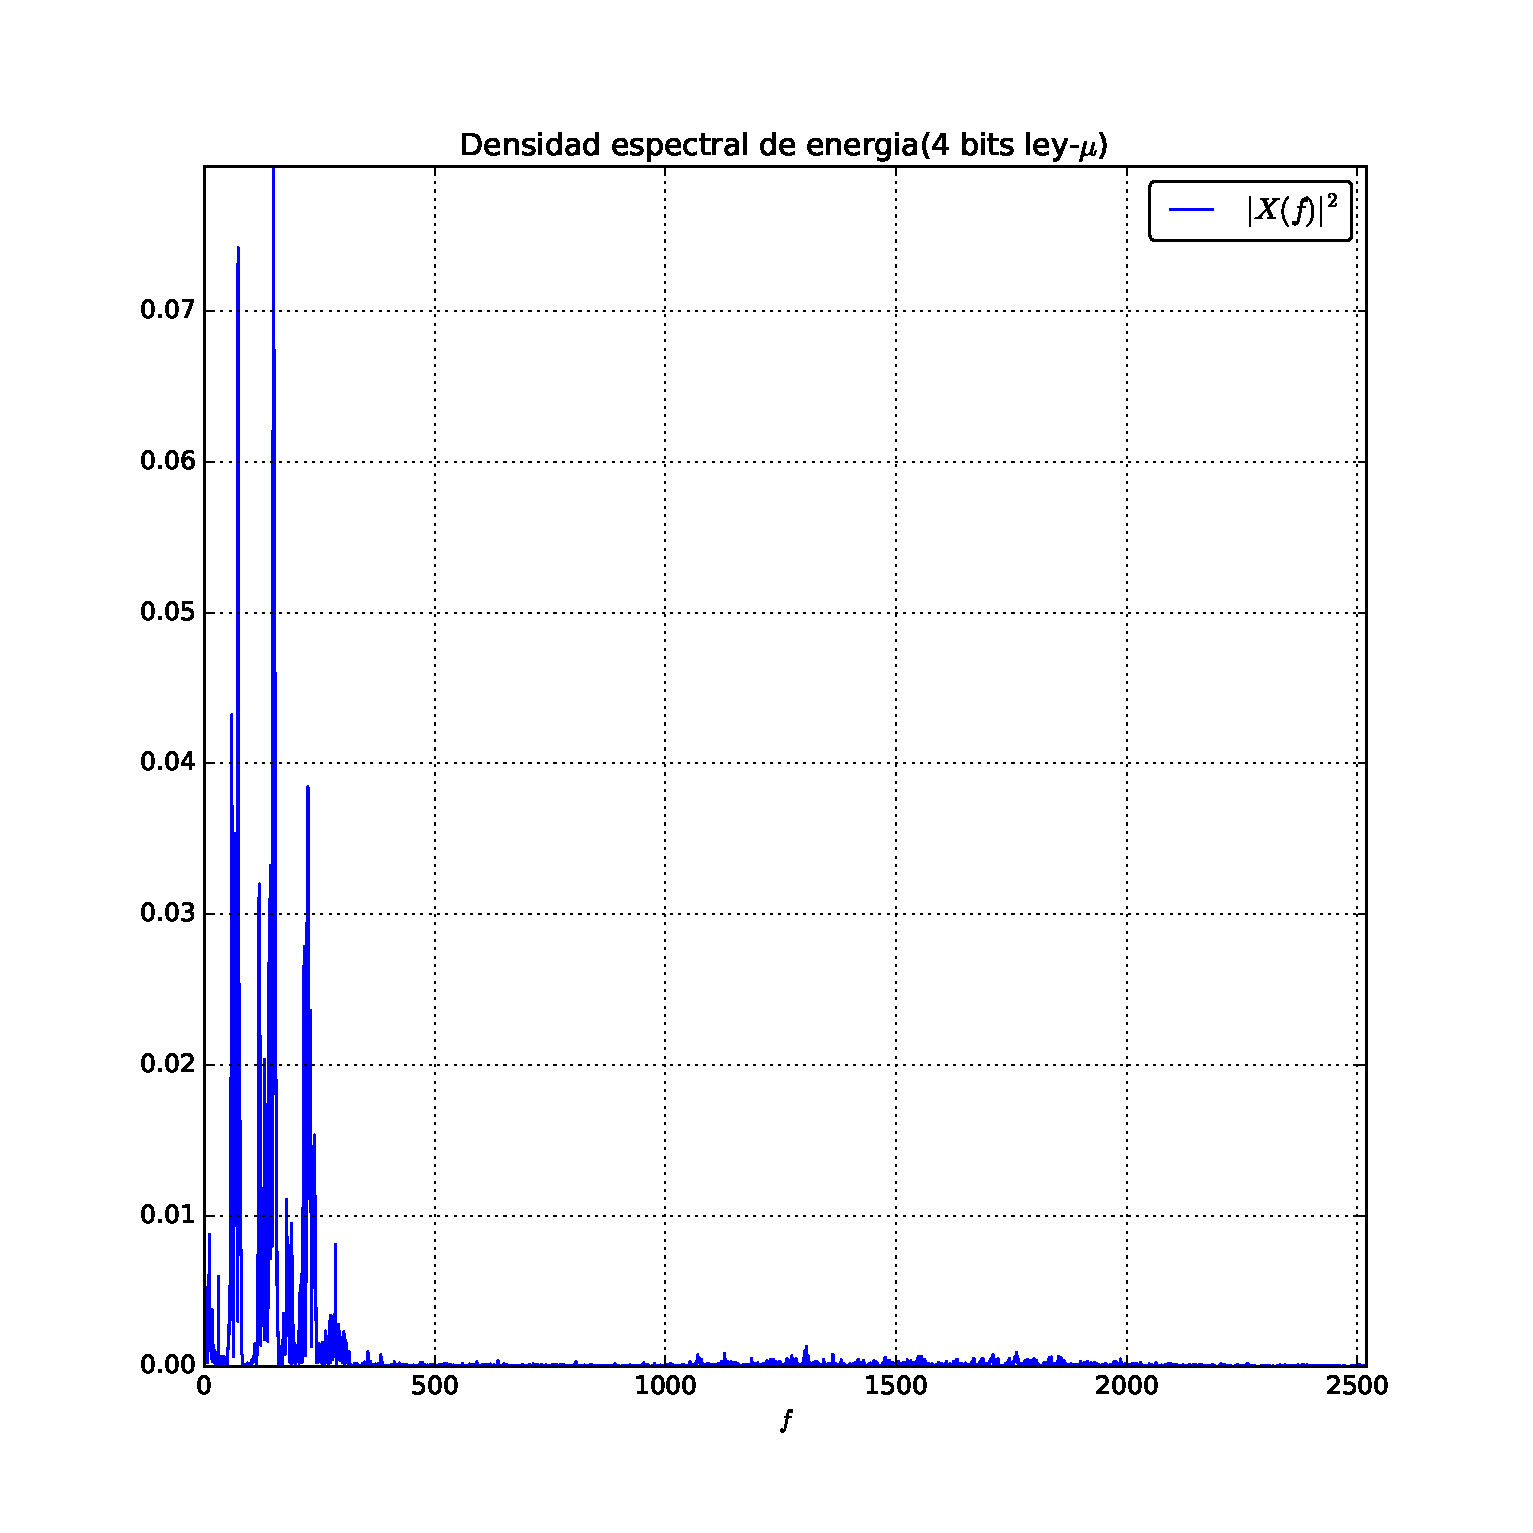
\includegraphics[width=0.48\textwidth]{./Images/densidad_espectral_x_4.eps}
   \caption{densidad espectral energia 4 bits}\label{fig:densidad_x_4}     
\end{figure}

Vemos que se mejora la relacion senial-ruido como esperabamos ya que se trata de 
una senial de voz y la ley de compresion $\mu$ esta pensada para estas seniales.

\section{Problema 7}

Dada los siguientes pares de señales, añada ruido y pruebe el comportamiento
del filtro adaptado para la deteccion de las mismas.
\begin{displaymath}
   S_{1a}(t) = \left\{
     \begin{array}{lr}
        A & : 0 < \, t \, < \frac{T}{2} \\
        0 & : \frac{T}{2} < \, t < \,T \\
     \end{array}
   \right.
\end{displaymath} 
\begin{displaymath}
   S_{1b}(t) = \left\{
     \begin{array}{lr}
        0 & : 0 < \, T \, < \frac{T}{4} \\
        A & : \frac{T}{4} < \, t < \,\frac{3T}{4} \\
        0 & : \frac{3T}{4} < \, t < \,T
     \end{array}
   \right.
\end{displaymath} 
\begin{displaymath}
   S_{2a}(t) = \left\{
     \begin{array}{lr}
        A & : 0 < \, t \, < \frac{T}{2} \\
        0 & : \frac{T}{2} < \, t < \,T \\
     \end{array}
   \right.
\end{displaymath} 
\begin{displaymath}
   S_{2b}(t) = \left\{
     \begin{array}{lr}
        0 & : 0 < \, t \, < \frac{T}{2} \\
        A & : \frac{T}{2} < \, t < \,T \\
     \end{array}
   \right.
\end{displaymath} 
\begin{displaymath}
   S_{3a}(t) = \left\{
     \begin{array}{lr}
        A & : 0 < \, t \, < \frac{T}{2} \\
        0 & : \frac{T}{2} < \, T < \,T \\
     \end{array}
   \right.
\end{displaymath} 
\begin{displaymath}
   S_{3b}(t) = \left\{
     \begin{array}{lr}
        -A & : 0 < \, t \, < \frac{T}{2} \\
        0 & : \frac{T}{2} < \, t < \,T \\
     \end{array}
   \right.
\end{displaymath} 

\subsection{resolucion}
Nuevamente se realizó un script(\verb|problema7.jl|) que realiza 
y además comparamos gráficamente todas las seniales. A continuación las salidas del mencionado script.

\begin{figure}[H] 
\centering
   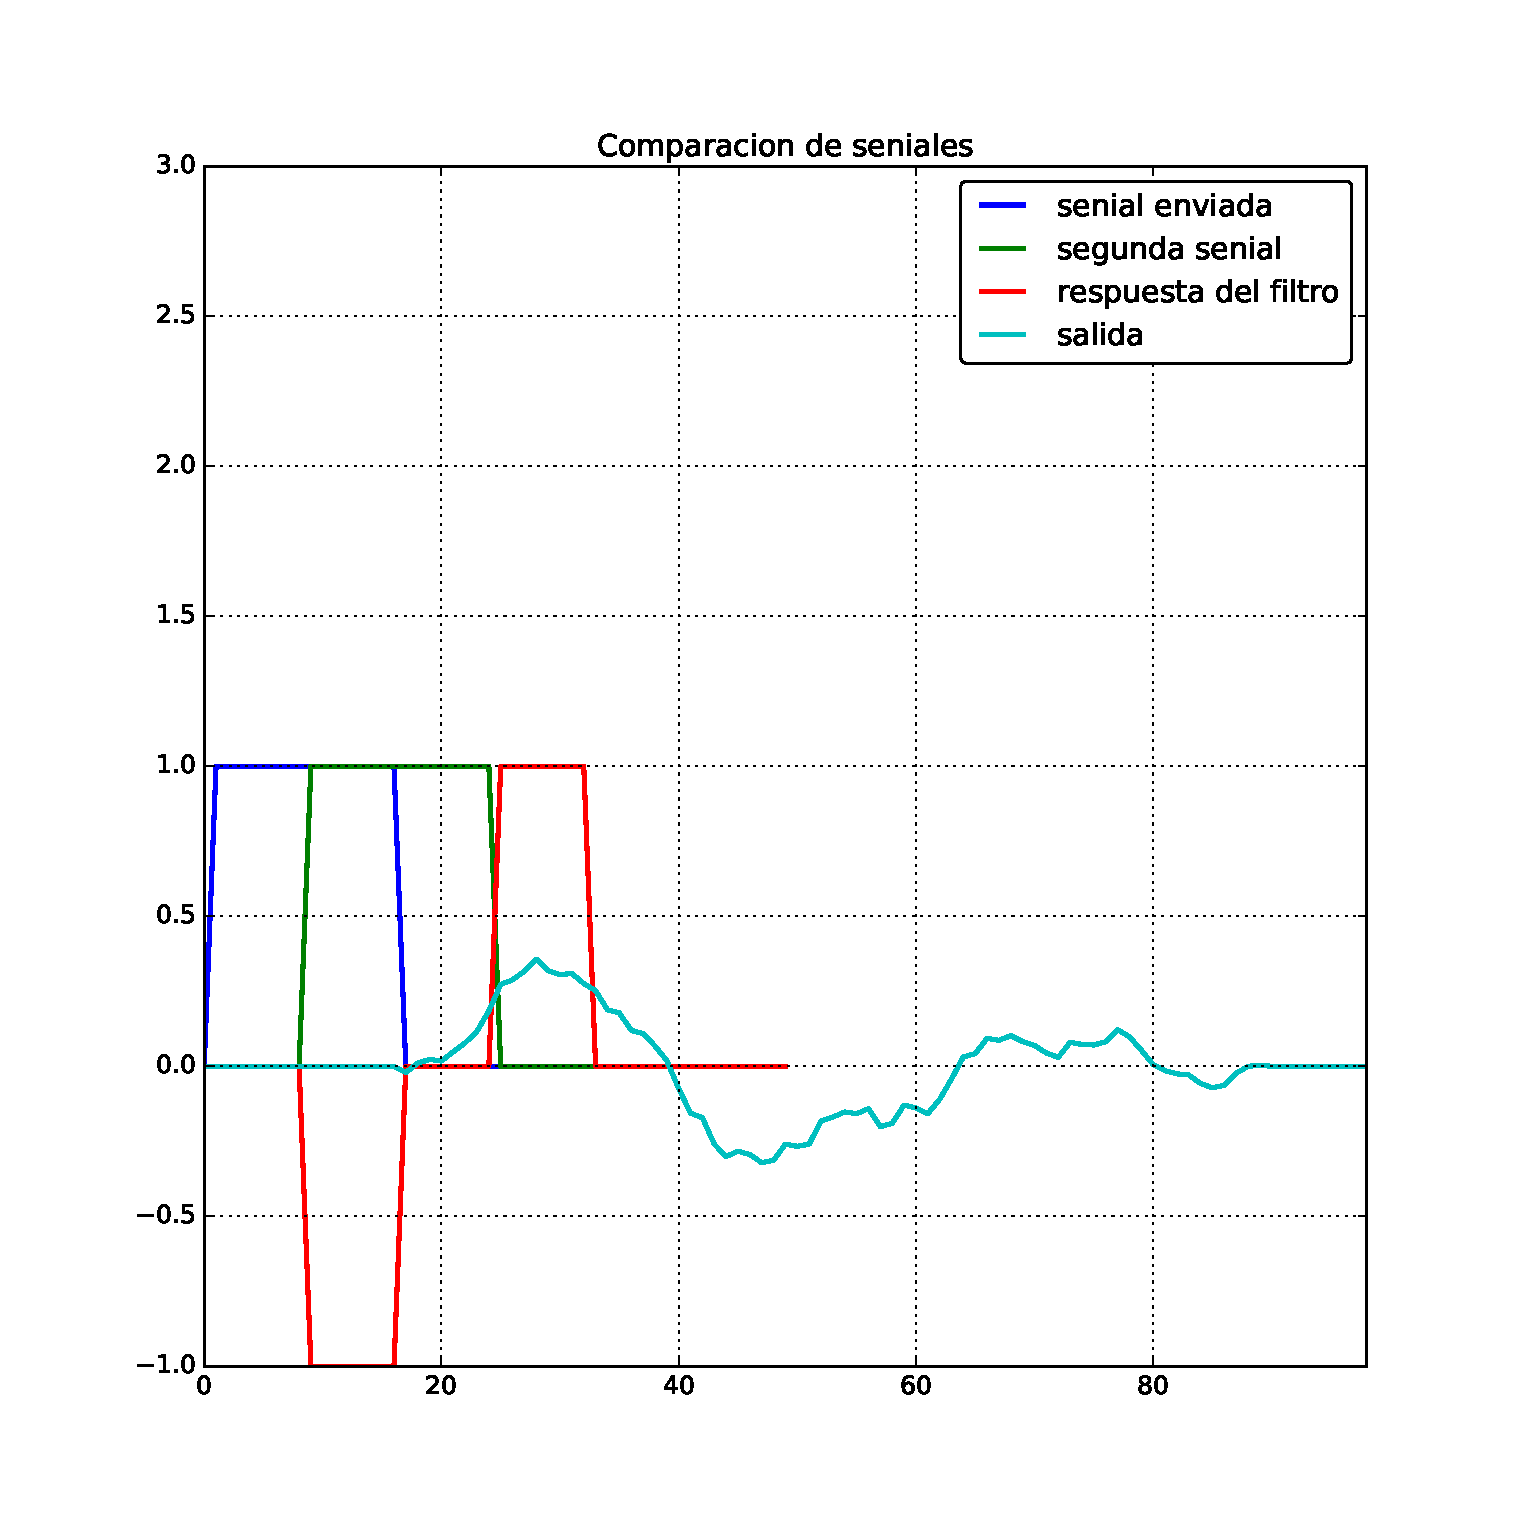
\includegraphics[width=0.48\textwidth]{./Images/filtro_adaptado1.eps}
   \caption{salidas del filtro adaptado para el conjuinto 1}\label{fig:filtro_1}     
\end{figure}

\begin{figure}[H]
   \centering
   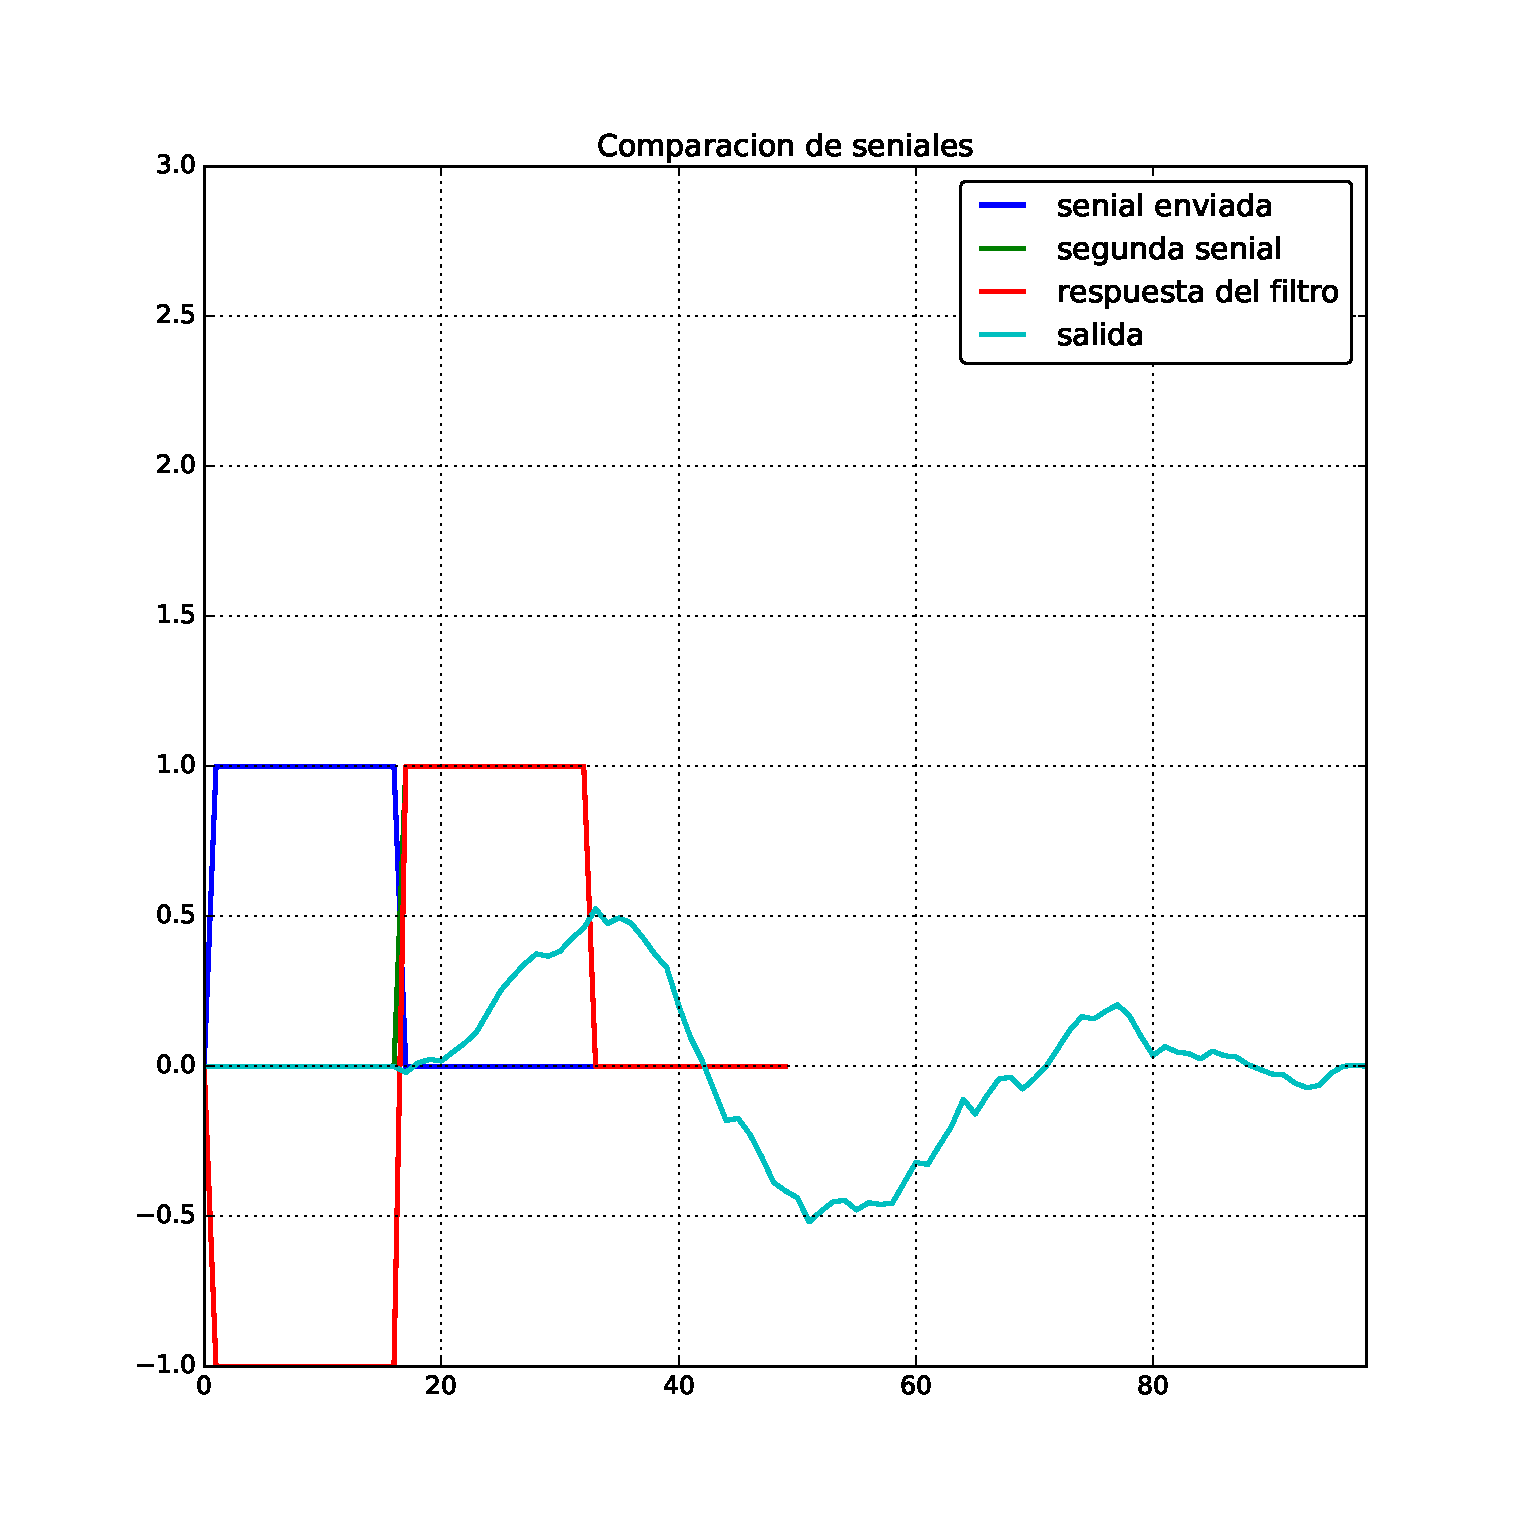
\includegraphics[width=0.48\textwidth]{./Images/filtro_adaptado2.eps}
   \caption{salidas del filtro adaptado para el conjuinto 2}\label{fig:filtro_2}     
\end{figure}

\begin{figure}[H]
   \centering
   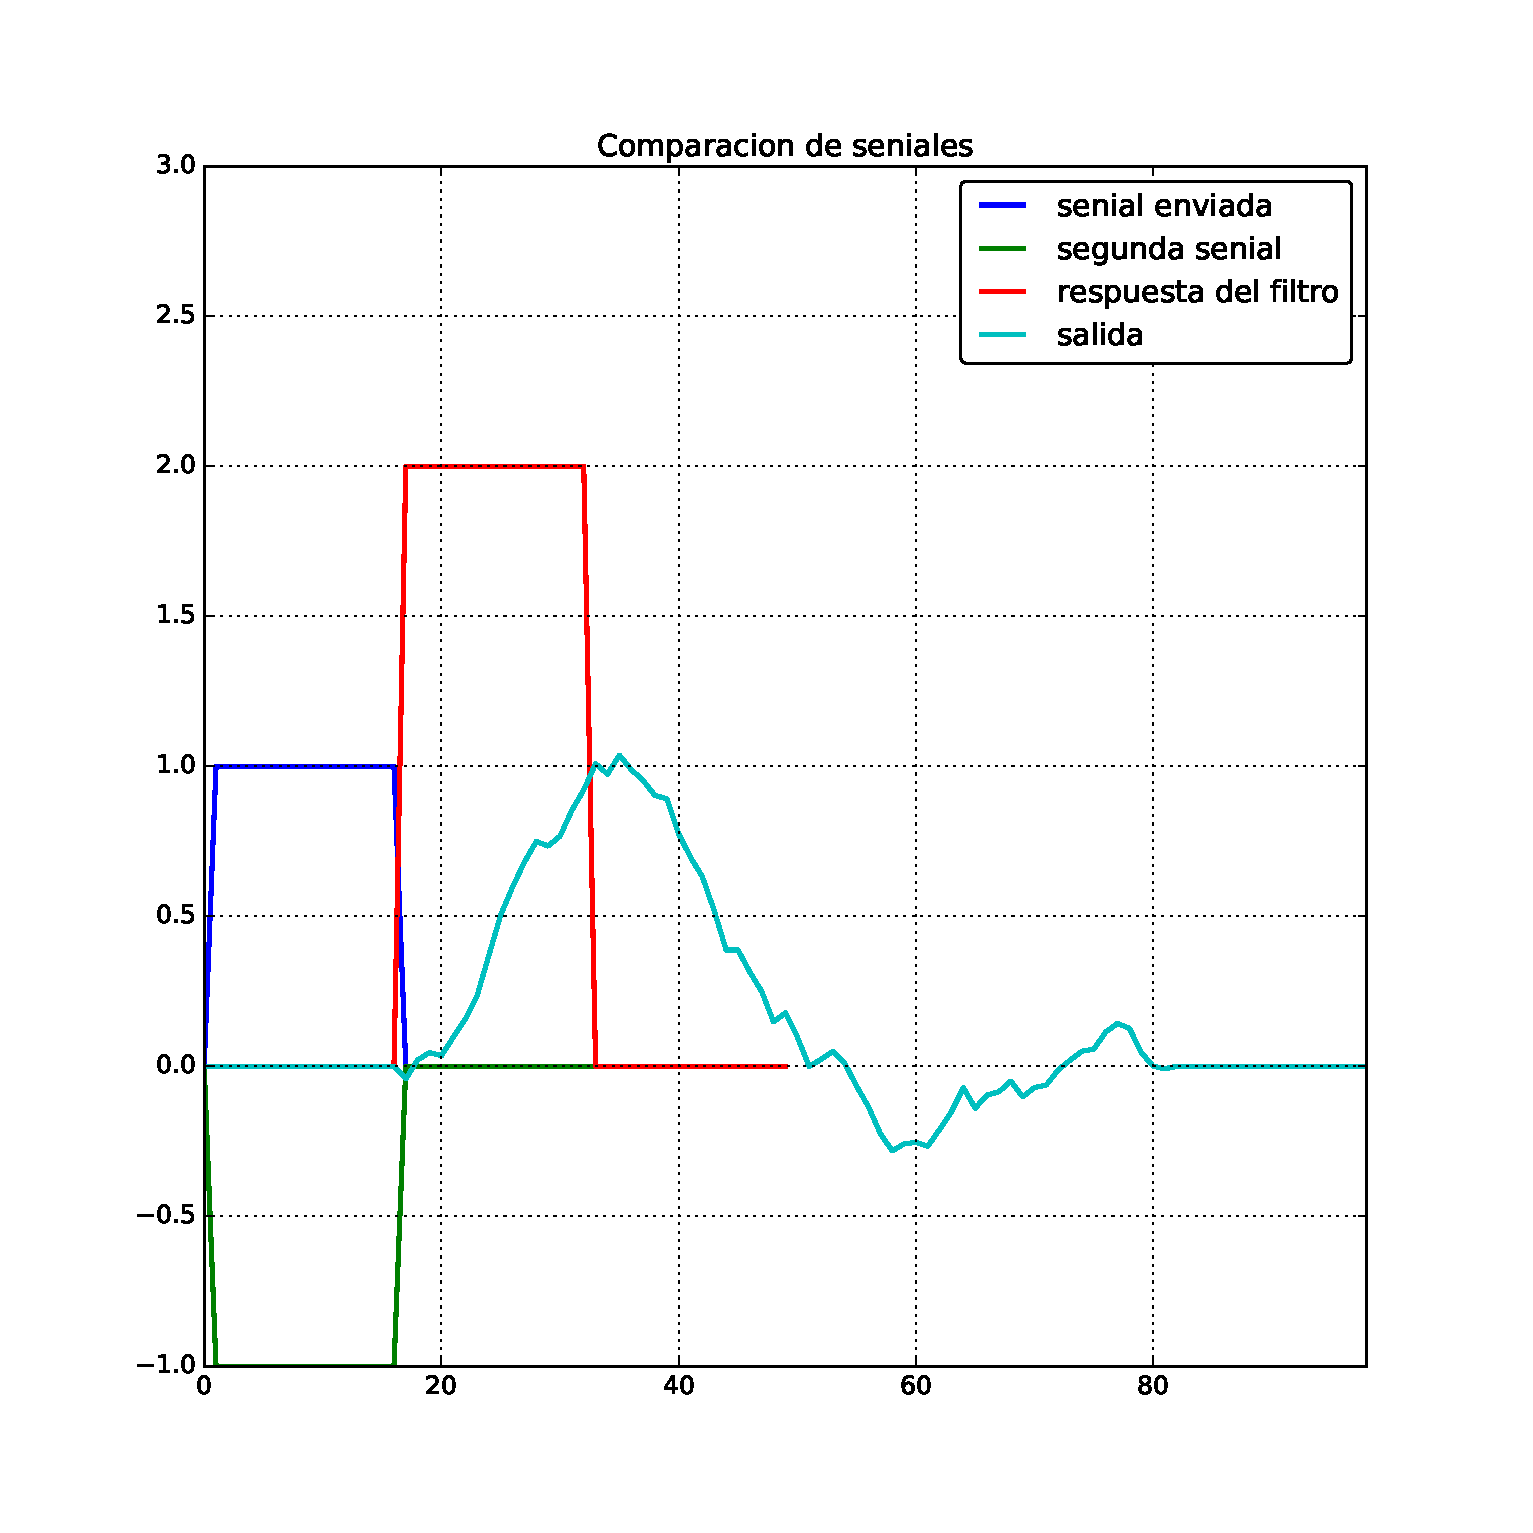
\includegraphics[width=0.48\textwidth]{./Images/filtro_adaptado3.eps}
   \caption{salidas del filtro adaptado para el conjuinto 3}\label{fig:filtro_3}     
\end{figure}


Vemos que el conjunto 3 que es una senial bipolar se comporta mejor, como esperabamos 
ya que se puede transmitir con 3[db] menos de potencia a igual tasa de error de bit o 
probabilidad de error de bit.

\newpage 



%------------------------------------------------------------------------- 
% Bibliografia 
%-------------------------------------------------------------------------
\begin{thebibliography}{6} \bibitem{Principal}{Digital communications, fundamentals and applications. Bernard Sklar}\\ \bibitem{Principal2}{Julia: A fresh approach to numerical computing. Jeff Bezanson, Alan Edelman, Stefan Karpinski, Viral B. Shah(2014)}\url{http://arxiv.org/abs/1411.1607} 
\end{thebibliography} 

\end{document}
